\iflater\discuss{Maybe there are too many tasks???}\fi

\iflater

\todolast{GPG: Proposals should identify a computer and information
  science and engineering grand challenge and an agenda to tackle such
  a challenge.} \bcp{Check that we used the word ``agenda'' enough. :-)}

\todo{GPG: proposals should explain why existing CISE core programs
  for Small and Medium size projects
  (\$600,000 over three years and \$1,200,000 over four years,
  respectively) are inadequate to address the grand challenge. A
  strong rationale must be provided that explains why a budget of this
  magnitude is required to carry out the proposed work.}\bcp{We should
find a place to make this point explicitly.}

\todo{GPG: The proposal must explicitly identify the participating
  CISE core programs it covers and make the case for why the challenge
  is within the scope of one or more of these participating core
  programs.} \bcp{I put it in the Project Summary -- it's a bit
  clunky, but I think it serves.  And no one can say that we didn't
  satisfy the requirement!}
\fi

%% https://www.synopsys.com/content/dam/synopsys/sig-assets/reports/cpsq-report-nov-22-1.pdf

% \rjmh{ I think the *introduction* needs to
% identify work-in-progress/early results showing early payoff from the
% collaboration. "Bringing this combined expertise together has already
% enabled us to...". I think the reader needs to get (more) excited
% about the combination.
% }

% \todo{Incorporate something like this (from John):
%   \begin{itemize}
%   \item ``Software bugs are
%   notoriously commonplace; a 2002 report for Congress estimated their
%   cost to the US economy at almost \$60 billion per year—around
%   0,6\% of GDP. Software developers
%   devote around half their effort to testing their software, in order
%   to detect and eliminate most bugs before the software is
%   released. The same report estimated that improved techniques for
%   testing could save the US \$22 billion per year.''
%   \item ``In 2002, the National Institute of Standards and Technology
%   estimated the total cost of software errors to be almost \$60 billion
%   per year, in the US alone11. It follows that improved testing
%   techniques have the potential to save society very large sums; the
%   same report estimated that better testing infrastructure could save
%   \$22 billion of those \$60 billion, corresponding to 0.2\% of the
%   entire GDP of the USA at that time. Since then the volume of
%   software, and our dependence on it, has only grown. How much of
%   these savings can be realised using property-based testing is, of
%   course, a matter for speculation—but clearly, the problem PBT
%   addresses, of improving software quality, is critically important to
%   society as a whole."
%   \item The report: \url{https://www.nist.gov/system/files/documents/director/planning/report02-3.pdf}
%   \item Title of the report: The Economic Impacts of Inadequate
%   Infrastructure for Software Testing
% \item Harry's take: We need powerful tools like PBT because software
% bugs are expensive
% \begin{itemize}[noitemsep]
%         \item Bugs cost (\$60B/year in 2002 money)
%         \item It has been known since then that improving testing infrastructure is a critical way of driving that cost down
%         \item (Really wish we had more modern numbers)
% \end{itemize}
% \end{itemize}
% }


\section*{Project Description}

Testing plays a vital role in the robustness, security, and overall
quality of modern software. It comes in many styles---unit testing,
integration testing, performance testing, stress testing,
accessibility testing, penetration testing, etc.---supported by
diverse tools, with yet more advanced tools and methodologies always on
the horizon.

One such methodology is {\em property-based testing} (PBT),
sometimes described as ``formal specification without formal
verification.''  A developer characterizes the desired
behavior of
some piece of code in the form of executable {\em
  properties}. The code is
then validated against these properties by running it many times
with a large number of automatically generated test inputs.
%
% PBT thus achieves a comprehensiveness that is often not
% possible with alternative testing methods. \iflater\bcp{Why not with
%   fuzzing??  Can we say it explicitly, to avoid leaving a question
%   pending for some readers?}\fi
%
This combination of rich, high-level specifications and mostly
automatic validation has proven effective at identifying
subtle bugs in a wide variety of settings, including
telecommunications software~\cite{arts2006testing}, replicated
file and key-value
stores~\cite{MysteriesOfDropbox2016,Bornholt2021}, automotive
software~\cite{arts2015testing}, and other complex
systems~\cite{hughes2016experiences}.
It is used by companies including Amazon, Volvo, Stripe, Galois,
and IOG, which
runs the Cardano blockchain and the Ada cryptocurrency.

PBT took the functional programming world by storm following its
debut in the Haskell QuickCheck library~\cite{ClaessenHughes00}.  In
2010 the
QuickCheck authors received the ACM SIGPLAN ``Most Influential Paper of ICFP
2000'' for their paper describing it; this is currently the most cited
ICFP paper by
a factor of 2, according to ACM's digital library.  In the intervening
years, PBT has spread to many other software ecosystems:
%
Wikipedia lists QuickCheck variants in 40 programming languages, some
with several competing libraries~\cite{QuickCheckWikipedia} (Java alone has
7!).
%
And these libraries are popular:
the developers of the Hypothesis library in
Python~\cite{maciver2019hypothesis,HypothesisGithub} estimate its user community
at half a million~\cite{ZacPersonalCommunication,noauthor_python_nodate}.  On GitHub,
Hypothesis has 6.5K ``stars'' from developers, Rust's
quickcheck~\cite{RustQuickcheckGithub} has 2K,
ScalaCheck~\cite{ScalaCheckGithub} has 1.8K, and Clojure's
test.check~\cite{ClojureTest.checkGithub} has 1.1K.
By comparison, pytest, the main library Python users use to run
tests, has 9.6K stars~\cite{PytestGitHub}---i.e., Python's
PBT tool has around 70\% as many stars as Python's entire testing
infrastructure.

And there is still plenty of room
for growth.
The 500K estimate for
Hypothesis users is only 4\% of all Python developers; the Hypothesis
authors estimate that the ``addressable market'' for PBT is around
25\% of the Python
community, and that there remains significant room for
improving its usage by existing users.
Similarly, the list of
companies using PBT, while substantial, is very far from the whole of the software
industry.
These gaps represent a gigantic opportunity to increase software quality
and reduce software costs.
A 2002 study~\cn{}\amh{Missing citations; might need @BCP, I think I am missing
the email thread from rjmh to complete the reference}\hg{+1} estimated that the total cost of software errors is almost
\$60 billion per year and suggested that \$22 billion of that could be
saved through
better testing infrastructure; since then, the situation has only gotten worse, with a 2022
study~\cn{} estimating that poor software quality now costs over \$2 trillion per
year. Accelerating the adoption of PBT stands to make a
significant dent
in the global cost of software bugs.

Recognizing this opportunity, our group has been working to identify
high-leverage ways to extend PBT's reach.
In an ongoing need-finding study with PBT users at Jane Street
Capital, we found consistent enthusiasm---participants called it
``obviously valuable'' (Participant \participant{1}), built their own
libraries for it when standard ones were not available
(\participant{8}, \participant{21}), and suggested that ``everyone''
at the company should use it (\participant{20}); however, participants
also highlighted a key opportunity for improvement---{\em usability}. Like
many powerful tools, PBT can be difficult to apply, and developers
need support to do so effectively.

% \amh{This is a deficit-focused pitch---focusing on the problems that need to be
% solved with PBT---rather than an asset-focused pitch---focusing on how we need
% new paradigms for PBT. Can we shift the focus of this to stating one big way in
% which innovation in PBT is necessary?}
% Given all this momentum, one might wonder whether the research community
% has already discovered and addressed all of the challenges that might limit PBT's adoption
% in the broader software industry.  Sadly, it has not:
% in an ongoing need-finding study with users of OCaml's QuickCheck testing tool
% at Jane Street Capital, we have found
% consistent enthusiasm for PBT---participants called it
% ``obviously valuable'' (Participant \participant{1}),
% built their own libraries for it when standard ones were not available
% (\participant{8},
% \participant{21}), and suggested that ``everyone'' at the company should use it
% (\participant{20})---but participants also described {\em usability} issues that
% limit PBT's impact on the broader software community.

% Solving these issues
% requires advances in both technical foundations and
% tool design.\iflater\bcp{The last part of that sentence kind of
%   duplicates the first part of the next...}\fi

Improving the usability of PBT
requires insights from both the
programming languages (PL) and human-computer interaction (HCI)
communities.  On one side, PL provides conceptual background,
mathematical underpinnings, and established tools for PBT.  On the
other, HCI provides a deep foundation of theory and
practice for evaluating usability of systems in a
rigorous and objective way, including principled methods for
identifying problems, rigorous metrics, and proven
approaches to tool design---where tools, here, naturally include
``front end'' components like
data visualizers and IDE plug-ins, but
also ``back end'' technologies like domain-specific languages for
properties and generators; for the latter, HCI techniques
can help designers
strike the right balance between expressiveness and
accessibility~\cite{coblenz_pliers_2021,greenman_little_2022}.
Synergies like these led
Chasins et al.~\cite{chasins_pl_2021} to argue that a research
methodology combining PL and HCI hits a ``sweet spot'' where
need-finding techniques identify current
pain points, motivating concrete tools that help programmers write
safe, correct code.

% We intend to employ those particularly in the front-end aspect (the IDE for PBT);
% \item But also in the back-end (to strike the right balance between expressiveness and accessibility in our languages and libraries).
% \item For justification of the back-end language stuff, see the PLIERS paper
% % https://dl-acm-org.proxy.library.upenn.edu/doi/abs/10.1145/3452379
%  which provides a recipe for user-centered language design, and Little Tricky Logic
% % https://users.cs.utah.edu/~blg/resources/talks/vardifest-2022.pdf
% which argues that languages PL people like are often very confusing, and HCI methods can prevent us from designing languages that users won’t understand.
% \end{itemize}
% To provide tools for evaluating what we build that are faster and more direct than just putting things out into the world and waiting to see if users adopt them.

% Success in all these efforts will require complementary tools from PL and
% HCI research. HCI approaches will be used to concretely define
% developers' needs, design the user interface to tools, and evaluate
% their success, while PL techniques will be used to develop powerful
% domain-specific languages and type-based automation to improve the PBT
% process\proposecut{, as well as to formally validate these tools}.

Our team
is uniquely positioned to bring PBT into this vibrant area
of ``PL+HCI'' research.  PI Head recently
co-founded a new HCI group at
the University of Pennsylvania and specializes in interactive
programming environments, while PI Pierce has published widely on PL
topics including PBT.  Our past research collaboration has led to
two workshop
presentations~\cite{goldstein_problems_2022,shi_towards_2023} and to the ongoing
study at Jane Street mentioned above, which strongly informs the
research and technology transfer agenda for the present proposal.

\smallskip

We propose an interdisciplinary program of research and
engineering in
{property-based testing}, bringing to
bear the combined power of PL and HCI to accelerate PBT's transition
into practice.
%
Planned research,
engineering, and education activities can be grouped into five main
themes: \bcplater{This already feels too detailed, and we still need to write
blurbs for all the other tasks we've added in the past few days.  But
for now I think we should just go ahead and add stuff, and come back
later to presenting a grander summary.}
\hg{How is it looking now? I know this comment is pretty old}
\begin{enumerate}[noitemsep]
% \begin{itemize}[noitemsep]
% \begin{enumerate*}
\item We will establish a solid \thread{foundation} for HCI-informed research on PBT,
starting from our ongoing need-finding study. We will confirm
this study's findings and further explore usability of PBT via
two survey studies and an observation study
of PBT users {\em in situ} (\sectionref{sec:foundation}).
%
\item We will help developers efficiently define and tune random input
\thread{generators} with novel techniques for generating values
satisfying given preconditions, for test input mutation, and for
example-based generator tuning---all building on a novel
``reflective'' approach to generation (\sectionref{sec:gen}).
%
\item We will empower developers to \thread{specify} properties with new
languages for expressing properties, tools simplify the process of authoring
properties, and assistants that help to explain properties to others
(\sectionref{sec:spec}).
% tools for checking temporal properties over internal program states
% and for model-based testing of modularized code\proposecut{ and for authoring
% properties}, plus a comprehensive review of PBT practice to help
% students and developers identify situations where PBT is likely to be
% most useful\bcplater{the latter belongs under diffusion now, I
%   believe} 
%
\item We will build novel tools for \thread{interacting} with properties
and generators---helping developers locate the causes of test
failures and improve the distributions of randomly
generated test inputs to find bugs more effectively (\sectionref{sec:val}).
%
\item We will support the \thread{diffusion} of PBT tools and
methodologies from academia into industry through targeted engineering
---in particular, supporting and
improving open-source PBT libraries and building a comprehensive IDE for PBT.
We will also drive diffusion via education, developing materials to teach
software developers about high-value applications of PBT and materials for
undergraduate computer science curriculum centered around
PBT\bcplater{``centered around PBT'' is maybe a bit too grandiose...?}
(\sectionref{sec:diffusion}).  \iflater\bcp{Do we need to write explicitly about how education is key not only
to the diffusion area?  Or is this fine this way?}\hg{I think fine? But I'm not
totally sure}\fi
% \end{enumerate*}
% \end{itemize}
\end{enumerate}
%
The scale of this project---two PIs, four PhD students, and a staff
engineer---is essential to the success of (1) its
tightly integrated research agenda, which requires expertise across PL and
HCI to make significant advances in the five interconnected themes above, and (2) its
goal of broad impact on industrial
practice, requiring the full-time attention of a software engineer.
%
A detailed sketch of responsibilities and timeline can be found in the
Management and Coordination supplement, but, briefly,
one PhD student will build on our existing user studies to
develop a clear foundational understanding of
PBT from the perspective of usability and human factors, two students
will develop ``back end'' technologies to support usable
PBT workflows, and a final student will leverage these technological
advances to develop ``front end'' IDE support. The
research engineer will focus on transferring the
products of this research into an industrial context, supporting and enriching
existing open-source PBT projects with theoretically informed ideas
and tools. None of these
projects stands on its own; rather, each supports and informs the
others to achieve both conceptual advances and significant
impact on software development practice.
%
The Management and Coordination supplement also summarizes the metrics
we will use to monitor and measure success for the various project
tasks.

\forreaders{Please tell us whether you feel convinced, at this point,
  that we have articulated a compelling ``grand challenge'' and an agenda to
  address it.}

\forreaders{Also, please take an especially critical look at the
  Management and Coordination supplement and at what we say
  about coordination and management here in the main project
  description.  NSF cares a lot about this!}

Our plans for Broadening Participation in Computing, described in a
supplemental document, are focused in two areas: (1) expanding an
existing NSF-REU program that brings undergraduates from
underrepresented groups to Penn for summer research experiences in
programming languages, and (2) increasing diversity in the TA roster
for Penn's introductory computer science course.

\iflater
\bcp{Explain somewhere why it's grand... :-)  Specifically, explain why the
  resources of a Large grant are needed to address the challenge (why
  small or medium grants would not do it).}
\todo{Webinar: Proposals must be clear about why this kind of scale is
  required for the research to succeed.}
\discuss{Why do we need four PhD students---why can't this agenda be
  accomplished with fewer?  Why do we need an engineer?}
\fi

\medskip

The rest of this Project Description describes this research and
technology transfer agenda in detail.  Sections
\sectionref{sec:orientation} and \sectionref{sec:motivation} supply
background on PBT and present preliminary findings from our
ongoing study at Jane Street.
%
Sections \sectionref{sec:foundation} through
\sectionref{sec:diffusion} outline plans for each of the
themes listed above.
Section \sectionref{sec:broader-impacts}
discusses the Broader Impacts of the project, and
Section \sectionref{sec:prior} summarizes our prior
NSF-supported work.

\iflater\discuss{Can we come up with a good infographic for the
  introduction?}\fi

\iflater
\todo{GPG: ``Does the plan incorporate a mechanism to assess
  success?''  We need to talk about this explicitly!}
\fi

\SIMPLESECTION{Orientation: Property-Based Testing}{sec:orientation}

% We begin in this section with some background on PBT and preliminary
% results from our ongoing study at Jane Street

% \subsectionstar{Property-Based Testing}
% \subsectionstar{Orientation: Property-Based Testing}
%
PBT%
% , famously popularized by Haskell's QuickCheck library
~\cite{hughes2007quickcheck}
is software testing method where
executable functions are used as partial
specifications of a component under test. For example, a developer might
write the following property for an \lstinline{insert}
function on binary search trees, taking an arbitrary tree \texttt{t}
and an integer
\texttt{x} as parameters:
\begin{lstlisting}
  prop_insert_correct x t  =  (is_bst t ==> is_bst (insert x t))
\end{lstlisting}
That is, if the original tree
is a BST, then it should remain
a BST after the insertion of \texttt{x},
where \lstinline{is_bst} is a function that checks whether a binary
tree is arranged so that each node's label is greater
than any label in its left subtree and less than any in its right
subtree.
% \rjmhlater{The example property you give looks like a type check:
% given a BST as
% input, insert returns a BST as result. The reader may easily think
% such a property is of interest only in dynamically typed
% languages... and that it is a rather trivial property even there. Of
% course, I understand that it really tests that the BST invariant is
% preserved by insert, a deep semantic property, but you are just
% assuming that the reader will remember that binary search trees need
% to satisfy an invariant, and will guess that is_bst checks that
% invariant. Be more explicit to avoid a risk of misunderstanding. }%
In general, such a property is a function that
accepts a generated
test input
and evaluates to \lstinline{True} if the test passes and
\lstinline{False} otherwise.
% This one, ``\verb|prop_insert_correct|'',
% checks that an insert operation on a binary search tree preserves the
% binary ordering of the tree.
Given a property, the PBT tool generates a
large number of inputs and
checks that the property yields \lstinline{True} for each one; any input
that causes the property to fail is reported to the user as a
{counterexample}.

Our research agenda focuses mostly on {\em random}
generation~\cite{hamlet1994random}, the dominant approach in PBT,
though many of our tools would also be applicable to alternatives
like enumerative test-case
generation~\cite{DBLP:conf/haskell/RuncimanNL08, leancheck}.  The
surprising effectiveness of random generation can be attributed to the
``combinatorial nature'' of large test cases---the fact that bugs can
often be exposed by any test input that embodies some specific combination
of features, independent of whatever other features may also be
present.  For example, a bug might be triggered by a particular
sequence of API calls in a particular order, even when
these are interleaved with other API calls. As a result, testing with
large random inputs often exposes issues much faster than exhaustively
enumerating small inputs.  Techniques like swarm
testing~\cite{groce2012swarm} can further amplify this effect.

To apply PBT to a system or an individual software component, the
developer first defines one
or more properties that they expect should always be satisfied. Then
they supply {\em random input generators} for the values that the
properties take as input---these are sometimes written by hand, but
often they can be automatically generated, e.g., from the type of the
input. Next, they check their properties against many generated
inputs, using a test harness provided by their PBT tool. And finally, if
counterexamples are discovered, they inspect them to determine the
source of the bug.  Each of these steps can be significantly improved for users,
as we describe in the next
section.

\smallskip

Why go to the trouble of PBT, rather than the more straightforward
example-based testing that is standard across the software industry?
First and foremost because a component can be tested much more
thoroughly with a property plus many automatically generated examples
than with a small number of examples written out by hand.
% \proposecut{As mentioned
% previously, PBT has an impressive track-record uncovering bugs that other
% approaches had failed to
% find~\cite{arts2006testing,hughes2014mysteries,
% Bornholt2021,arts2015testing,hughes2016experiences}.}
But
PBT is more than just thorough---it is also more general than example-based
testing. For example, Wrenn et al.~\cite{wrenn2021using} observe that example-based testing
of programs whose correctness conditions are {\em relational} (e.g.,
topologically sorting a graph, which might
produce any of a number of correct results) is impossible to do
faithfully; a property-based specification is a better choice in
such cases.
PBT is also
an obvious choice if
the developer already has some semi-formal
specification in mind---for example if they are implementing behavior from an RFC or
other design document---because it provides a clear connection between the
specified behavior and the implementation.
Finally, the
properties required for PBT can also serve as documentation:
participants in our need-finding study (\participant{5}, \participant{21})
talked at length about properties being an ideal way to communicate what a
program is supposed to do.

PBT is also often compared to {\em fuzz testing} (or
``fuzzing'')~\cite{afl-readme}, which randomly tests software to find
vulnerabilities. Fuzzing is powerful, and we discuss ideas for bringing PBT and
fuzzing closer together later in the proposal
(\sectionref{sec:reflectivefuzzing}), but fundamentally modern fuzzers have
different goals from PBT. In general, fuzzers are run for a long time (hours or
days), testing the software from the outside in an attempt to find a crash
error. PBT, on the other hand, is part of the development process; properties
are run for much less time (on the order of seconds) and are aimed at finding
logical errors in smaller software components. Both techniques are useful, but
their approaches are applied in different ways, at different points in the
development process, to achieve different goals.

With all these advantages, one might hope to find PBT on every
software developer's toolbelt.  But PBT poses some challenges as well,
as we shall see next.

\SIMPLESECTION{Motivation: A Formative Study of PBT in Industry}{sec:motivation}
%
Our research agenda is strongly informed by preliminary findings from
an in-progress need-finding study at Jane Street Capital.  Our purpose
in this
study is to understand the usability challenges that must be addressed
to boost adoption of PBT in
industry. The study data consists of thirty semi-structured interviews
with (1) developers who use PBT and (2) maintainers of PBT tools.

Jane Street is
an attractive setting for several reasons.  First and most
importantly, PBT is
already well established there, so there is a large
population of people with well-informed opinions on its benefits and
challenges. Additionally, Jane Street famously builds much of its
software in OCaml, a mostly functional programming language with
a well-engineered PBT library. This unified
ecosystem ensures that developers have access to mature PBT tools,
experience using them in collaborative settings,
and awareness of language-level abstractions necessary
for advanced usage.

As of February 2023, the full complement of thirty interviews has been
completed at Jane Street and a preliminary round of qualitative
analysis is underway; full-scale analysis will begin later in the Spring.
Findings from the study will be disseminated in a submission to a
software engineering conference such as ICSE.  We also carried out a
smaller pilot study among Hypothesis users to prepare for the
full-scale study at Jane Street; its results were presented at the
2022 HATRA workshop~\cite{goldstein_problems_2022}.

\ifthemecolors\bcp{Make the colors here (if we're using them) match
  the ones in the timeline.  Also, we've got five main sections but
  only four colors here... is that confusing?  I think so.  Maybe
  better monochrome...}\fi
\newcommand{\proptheme}[1]{{\ifthemecolors\color{nord-orange}\fi \em #1}}
\newcommand{\gentheme}[1]{{\ifthemecolors\color{nord-green}\fi \em #1}}
\newcommand{\evaltheme}[1]{{\ifthemecolors\color{nord-purple}\fi \em #1}}
\newcommand{\edutheme}[1]{{\ifthemecolors\color{nord-frost4}\fi \em #1}}

\subsectionstar{Usability Challenges}\hg{Is this section header doing anything?} The final product from
the ongoing study will be a fine-grained, qualitative description of how
Jane Street developers use PBT, what they need from it, and how the
research community can
help improve it.  While the full analysis of the interview data remains
to be completed, a number of themes are already clear; these
% , together
% with the findings of the preliminary study,
form the backbone of the present proposal. We describe them below,
italicizing themes, and
referring to evidence from participants in the Jane Street study
(\participant{1--30})
and the pilot study (Pilot-\participant{1--8}).

One set of themes concerned the \thread{generation} of
random inputs for PBT. Developers spoke
highly of the \gentheme{Derived Generators} that can be automatically
inferred from
the OCaml type system (\participant{5} called OCaml's tools for this
``[expletive] amazing'' and \participant{30} called them a ``game changer'').
These generators are already quite good, but they could be better: participants
identified deficiencies both small and large, e.g., for example, the fact
that derived generators
cannot enforce semantic preconditions like \lstinline{is_bst}.\amh{Question from
Elena: is this issue small or
large?}


When derived generators
failed, participants fell back to \gentheme{Bespoke Generators}, which
are far more flexible but proportionally more time-consuming to
build. For example, \participant{20} successfully used a bespoke
generator for XML documents to find significant bugs in their code,
but reported spending ``at least a day'' writing it.
Improving the abstractions available for authoring bespoke generators would
greatly improve the usability of PBT.
%
When a generated input turns out to be a counterexample that triggers
a property violation, the developer will need to inspect that
counterexample to find
and fix the root problem. Developers often implemented code for
\gentheme{Shrinking} counterexamples to discover
simpler inputs that trigger the same bug.  \participant{8}
and \participant{21}, who each implemented their own PBT libraries, both
incorporated shrinkers as key components. But
shrinkers need to be customized to particular kinds of data to be most
effective, and they can be time-consuming to build; several
developers
(\participant{16}, \participant{20} \participant{21}, \participant{30})
described constructing shrinkers as an opaque and difficult process.
% Ideally, developers would have tools that make the process of implementing
% shrinkers fast and simple.

A different set of themes
themes revolves around properties themselves, i.e.,
\thread{specifications}.
% and the kinds of programs in which they choose to test them.
PBT is often described as a lightweight formal method, and one
might therefore imagine that a common challenge would be coming up with the
specifications of desired program behavior. Indeed, in our earlier pilot
study~\cite{goldstein_problems_2022}, some respondents indicated just that:
developers with less experience with PBT
sometimes struggled to \proptheme{Imagine
Properties} or to understand what properties to test (Pilot-\participant{1},
Pilot-\participant{3--5}).
By contrast, Jane Street developers on the whole reported
little difficulty finding
properties. Rather, most developers applied PBT in
\proptheme{High-Leverage Scenarios} where properties were already
available or straightforward to invent. In the words of
\participant{9}, PBT is particularly easy to apply
when
one has ``a really good abstraction with a complicated implementation.''
When asked to speculate, several participants (\participant{3}, \participant{15},
\participant{20}, \participant{22}) guessed
that 80--100\% of Jane Street
developers write programs like this,
% \bcplater{Did anyone really guess
%   100\%??}\hg{Yep! Someone said ``everyone.''}
where properties are easy to find and
PBT is relatively easy to apply. This suggests that an effective way to
boost PBT in industry would be to provide
educational materials and documentation that highlight
real-world applications where it is a natural
fit.

We also heard \proptheme{Opportunities for Better
Leverage} of specifications, where PBT is not easy {\em yet} but
could be with a bit more research effort. For example, developers in
both studies (Pilot-\participant{4--6} and Jane Street \participant{7}) complained
that PBT was difficult when code was poorly abstracted.  Further,
more than three
quarters of study participants had used a particular approach to PBT commonly
called \proptheme{Model-Based Testing}.  \participant{3}, an author of PBT tools
at Jane Street, considered better automation and tooling around model-based
testing to be one of the most significant ways to improve PBT usability.


A further set of themes concerned the
\thread{interaction} between developers and their
testing environments---especially the processes they use
for \evaltheme{Evaluating the
Effectiveness} of their tests. Many
wished for
better ways to evaluate their generators and properties, including
feedback on code coverage (\participant{9} and \participant{25}),
mutation
testing~\cite{papadakis_mutation_2018}, and help understanding the
distribution of randomly generated
inputs (\participant{10}, \participant{16}, \participant{16}). Problematically,
while many developers admitted they would benefit from better tools for
evaluating their tests, many seemed to
\evaltheme{Implicitly Trust the Infrastructure} that they did use. \participant{14} actually shipped broken code because
they did not realize their generator had missed important input
examples.
Additionally, one participant (\participant{14}) saw significant benefit from
\evaltheme{Visualizations} and other tools that they had built themselves to
understand their testing effectiveness.

Finally, our experience with these studies (and with the products of
our own prior research!) suggests
that significant engineering and pedagogical effort is needed to amplify
PBT's \thread{diffusion} into the broader community.  Developers in both studies
(Pilot-\participant{1}, Pilot-\participant{4}, JS \participant{3} and
\participant{11}) reported a dearth of \edutheme{Documentation and Examples} for
learning about PBT.  PBT is also not
taught in traditional computer science curricula; making more developers
aware of it will required expanded
\edutheme{Classroom Education}. Finally, existing tools for PBT need continual
support to meet demands from increasing user-bases; if PBT is to become mainstream, we
need to offer \edutheme{Support and Guidance for Open-Source
Libraries}\hg{BCP feel free to suggest a new name here---I changed ``communities''
to ``libraries'' but I'm still not attached to the theme}
to help our
work and ideas permeate the PBT world.

The work throughout the rest of this proposal is inspired, in part, by these
motivating themes.
% \iflater
% \bcp{Needs a rewrite for the new structure... Section 7 is missing!
%   Or maybe we can just drop this paragraph?!}%
% %
% We discuss plans for work that addresses \proptheme{specification
%   themes} in \sectionref{sec:spec}, \gentheme{generation themes} in
% \sectionref{sec:gen},
%   \evaltheme{validation themes} in \sectionref{sec:val}, and \edutheme{diffusion
%   themes} in \sectionref{sec:ed}.  To support all of this work,
% \sectionref{sec:foundation} describes plans for a further round of
% studies to deepen our understanding of PBT needs and opportunities
% across a wide range of industrial settings.
% \fi

\SECTION{Foundation}{Understanding Needs and Opportunities%
\pagebudget{1}}{sec:foundation}

\iflater\todo{Mention how time-consuming these studies are (give some
  numbers and details).  We've allocated one whole PhD student to this
  aspect of the work.}\fi

The ultimate findings from the Jane Street user study\iflater\bcp{We call
  it a user study here, a need-finding study above, and I think a
  foundational study somewhere.  Let's rationalize this.}\fi{} should
give us a clear
picture of the benefits and challenges of PBT in the specific context
of Jane Street and other organizations with similar characteristics.  But to
fully understand the potential impact of PBT across the whole software
industry---as well as the factors that may limit its adoption---we need to
cast a wider net.
%
In this section, we describe four planned studies that aim
to produce a comprehensive, actionable
agenda for the latter stages of this project and beyond.  We plan two
written surveys, one to assess the generality of these needs and obstacles
and one to identify potential for adoption of PBT tools
(\sectionref{sec:survey}), a design study using a minimal PBT
framework (\sectionref{sec:frameworks}), and an observation study to understand
particular tasks involved in PBT, to guide the design of
interactive tools
(\sectionref{sec:observations}). Finally, we plan to distill these
study findings into a cognitive
theory of property-based testing, a conceptual foundation for the
design activities elsewhere in the project (\sectionref{sec:cogtheory}).

\bcplater{Not sure exactly how to phrase it, but we need to emphasize
  (probably repoeatedly) that these studies all require significant
  effort, and that all of them together will yield enough papers to
  make up a dissertation.  This will be clear to HCI folks, but not
  PL folks.}

\SUBSECTION{Generalizability of the Jane Street findings}%
   {sec:survey}{1}{2}{HCI Theory}{PhD 1}{}{Head}
%
Preliminary findings from the Jane Street study have already revealed
a number of
opportunities to improve property-based testing. To identify
others and better understand which are most
critical, we will conduct two
surveys with broader samples of developers. These surveys aim to
(1) determine which obstacles observed in the interview
study\iflater\bcp{sigh: another term :-)}\fi{}
represent widely experienced pain points and
(2) understand the potential benefits of better tools for the
software industry as a whole.

% \TASK{Validation survey}{1}{1}{Who?}
The main survey
aims to confirm (or perhaps refute) that
the things we are learning from Jane Street generalize to other settings.
We will
ask developers which of the issues we found at Jane Street are
ones they have also encountered, which are most severe
in their experience, and which
other issues they have encountered.
To provide
clear usage scenarios, respondents will
be asked to write brief anecdotes elaborating on the
most severe issues they remember.  Other questions will assess how
heavily respondents depend on specific features of their PBT tools
that may be enabled by their
ambient programming environment and language, e.g., whether their
language supports Haskell-like typeclasses or OCaml-style
metaprogramming, both of which are used to good effect by
PBT tools in those languages. 
Respondents will
be recruited broadly, from three main sources: (1)
users of the Python Hypothesis framework; (2) Jane Street, aiming for
a broader set of developers than in the interview study; and (3)
word of mouth and via announcements on the PIs' Twitter and Mastodon
accounts, various mailing lists, and discussion boards for developer
conferences---e.g., ``Yow!'', where PI Pierce spoke last
year~\cite{Pierce:Yow22}. We are aiming for   \bcplater{How many respondants are we
  aiming for??} \amh{I clarified this below}
% Types and types-announce mailing lists. They are mailing
% lists for the types programming. We will distribute announcements among
% attendees of conferences like ICFP or ``Yow!'' whom have
% a cumulative thousands of programmers with functional
% programming experience.
In line with typical practice in 
human factors research surveys in software
engineering~\cite{ref:robillard2009makes,ref:uddin2015api,ref:murphyhill2019predicts},
we aim to recruit respondents in the low hundreds (i.e., between 75 and 300
respondents) for each survey.

% \TASK{Impact survey}{2}{2}{Who?}
A second, more speculative, written survey later in the project will investigate
how broadly PBT may {\em eventually} be able to reach.  To get a sense
of this, we will
survey ``proximal'' users of PBT---developers who do not use PBT
currently but who might find it particularly
useful.
\proposecut{Particular attention will be given to those whose work requires
writing validation code and public APIs with some definition of types\bcp{Huh?}.}
We
will again recruit a broad sample of participants from varied settings
(professional, open source, educational) by working with our industry contacts
and recruiting over social media.
%
\proposecut{This survey will be more
difficult to ``get right'' than the first, and its design will
accordingly evolve over time as we gain a
better understanding of situations where PBT is most effective
(see \sectionref{sec:whento}), but we believe it can provide invaluable
feedback to PBT researchers about how far their work can reach.}
\iflater \hg{We should be more confident with this task---we're asking for
plenty of money, let's do it.} \bcp{+1} \fi

% \SUBSECTION{Usability of PBT Frameworks}%
\SUBSECTION{Dimensions of PBT infrastructure design}%
  {sec:frameworks}{3}{4}{HCI Theory}{PhD
1}{PhD 4}{Head}
%
Anecdotes related in interviews do not, in themselves, provide enough
information to inform the design of effective tools.  We will need a more
fine-grained understanding of the design trade-offs inherent in PBT frameworks
in order to improve those frameworks.  \bcplater{We use ``tool'' and
  ``framework'' interchangeably here (and I guess elsewhere?).  Are
  they really synonyms?  Is this confusing?}
Of course, a pairwise comparison of {\em all} frameworks in {\em all}
languages would be infeasible and
unhelpful; rather, we will systematically review prior art to identify major
dimensions along which PBT frameworks differ. For example, some frameworks, like
OCaml's QuickCheck, lean heavily into automating random data generation, whereas
Haskell's Hedgehog is designed to be more manual in the hopes of
making users more intentional about their testing... which of these approaches is
preferable? Similarly, some frameworks implement properties as arbitrary
host-language functions, while others provide a rich domain-specific language of
properties... do such property languages make a positive difference?

We will evaluate how differences along those dimensions impact usability in
two ways. First, we will design and implement a minimal, modular PBT framework
that can be tuned along the dimensions we want to study.  \iflater\bcp{Can we
give a bit more detail about what this language will be like?  How is it related
to the ``Reference implementation'' idea we talk about elsewhere?}\fi We will
then give users testing tasks and measure the speed, effectiveness, and
confidence with which they performed their testing.  Second, we will compile a
list of representative testing scenarios and interview expert users on their
preferences along the different dimensions for those specific tasks. This will
help us identify potential confounding factors in our other evaluation and add
depth to the analysis of how different workloads impact user's preferences.  In
this way, we will generate design recommendations that we can use as evidence to
help the community standardize on usable designs.

\bcp{I am not really convinced by this yet.  What are these
  ``dimensions'' where we are going to choose between alternative A
  and alternative B?  Integrated vs. external shrinking, sure, but
  after that, what??  If we can list four or five key dimensions, we
  should.  If not, maybe drop this task?  (I'm also worried about how
  easy it's going to be to implement a new PBT tool that embodies all
  possible combinations of these choices, much less in a ``minimal''
  way...)}\hg{I listed three, internal vs external shrinking, maximal vs minimal
  generator automation, and bespoke property language vs. just write a Boolean
  function. I imagine we'd find more if we actually did the study... My goal
  with this project would be to have an empirical basis on which to say ``hey
  QuickCheck, let's just implement internal shrinking'' and ``hey Hedgehog, you
  may want to give users better generator automation.'' It's consistently
  frustrating when a library in one language is strictly better in one way, and
  one in another language is better in another, and it has nothing to do with
  the language}

\SUBSECTION{PBT interaction models}{sec:observations}{4}{5}{HCI
   Theory}{PhD 1}{}{Head}
%
Our higher-level studies explore larger-scale usability challenges, but in order
to build usable tools we also need to know about the low-level interactions that
take place between users and their PBT systems. Understanding user interactions
is a core activity of HCI research and helps to inform robust interface design.

As a basis for designing tools with novel interfaces (see
\sectionref{sec:val}), we will observe developers working on PBT tasks.
Observations are time-consuming, both to perform and especially to analyze,
since they generate large amounts of subtle data, but they are the only way to
answer critical questions like:
(1) How much time
are participants willing to devote to
creating a property or tuning a generator when in the
middle of a programming task?
(2) How much space is available on a developer's
screen (amidst other tools like code editors and terminals) for
new
interfaces? and
(3) What are developers' current strategies for solving the
problems they describe---e.g., what representations of generated data
seem most helpful
for a programmer trying to understand the distribution of data generated by a
generator?

Observations will allow us to evolve singular anecdotes from the interview study
into a more comprehensive picture of the kinds of designs that will help
programmers.  We can avoid wasting significant time and energy building
interfaces that are unacceptable to users if we put in this work up front to
understand user workflows.  We ultimately plan to use this data to design tools
that give as much power as possible to users willing to invest more effort but
that also provide significant value ``for free'' to new users.

\bcplater{This is the one where I am least confident that PL reviewers
will be able to see where the effort would go in such a study (i.e.,
why it's a top-level task).}\hg{Any better?}

\SUBSECTION{A cognitive theory of PBT}{sec:cogtheory}{2}{3}{HCI
  Theory}{PhD 1}{Everyone}{Head}
%
A cornerstone of our efforts to bring usable PBT to more people
will be a new theory of property-based testing itself.  Theories of
programming have
long served a critical role in human-centered software engineering
research, providing rich and memorable descriptions of programming
processes and clarifying opportunities to improve tooling and training.
For instance, the {\em information foraging
  theory}~\cite{ref:lawrance2010programmers}
describes how programmers navigate a complex code base in search of behaviors
within the code and helps understand why programmers sometimes fail
in this task. This
theory has motivated a variety of tools that demonstrably improve the
programming experience (e.g.,~\cite{ref:henley2014patchworks}).  Other theories
that have inspired advances in programming tools include
Blackwell's Attention-Investment model~\cite{ref:blackwell2002first} Ko and
Myers' debugging framework~\cite{ref:ko2005framework}, and Ko's characterization
of end-user programming barriers~\cite{ref:ko2004six}.

Recognizing the power of theory, one of the first steps in our
research will be to develop a theory of property-based
testing. The starting point
will be the conceptual framework we are developing through the Jane Street study. This
will be validated and refined through contextual inquiries with
programmers~\cite[Ch.~3]{ref:holtzblatt1997contextual}\bcp{explain}, leading to a provisional
theory during the first two years.  This theory will help us
refine our ideas for
tools and provide a foundation for contextualizing the questionnaires and
observations described in the following sections. Conversely, evaluations of
the tools we build will provide additional evidence to further
refine the theory.

\bcp{The specifics of the theory that Andrew had sketched seem too
  contentious (I think especially PL people will be distracted by
  trying to figure out whether they believe them), but I do think we
  need a short paragraph giving a bit more detailed impression of what
  the elements of such a theory might be like.  E.g., what's its
  success criterion?  (All of these tasks could use some discussion of
  success criteria, in fact!)}

% In the rest of this section, we sketch the outlines of a speculative
% theory that could
% follow from the Jane
% Street study.
% While the theory we ultimately develop may well look quite different
% from this, we
% describe it here to demonstrate what such a theory might look like and
% suggest some of its predictive
% potential.
% We call it the \emph{hill-climbing} theory because (on this reading)
% PBT can be thought of as following a hill-climbing process: a
% property-based test
% is developed through a series of steps, each consisting of either
% refining the specifications or refining the generators\bcp{I'm
%   not very sure I believe that.}. In contrast to
% conventional software development, when operating with this climbing
% perspective, a programmer is
% constantly adjusting course when a step is too ``steep,'' i.e., when it is not
% easy to refine the specification or generator.\bcp{Why would this be?
% (What kinds of refinements are they trying to make?  What determines
% when they are easy or hard?)} Programmers stop climbing when
% they feel they cannot make progress. Accordingly, for a programmer to develop a
% powerful test suite, they need to be supported in incremental, low-cost
% refinements of both specifications and generators, with the ability to quickly
% determine whether they have in fact progressed.

% The value of this theory is in part what it implies about PBT tools.
% Tools should make it possible to ``cover a lot of ground,'' i.e., test a
% large amount of significant program behavior, without a lot of work. They must
% to support rapid progress, because programmers' tend to invest minimal effort
% investigating paths they consider to be unfruitful in automated testing.
% Programmers can be aided by either helping them with ``way-finding'' (i.e.,
% teaching them strategies for refining specifications and generators to better
% test their systems), or with better ``equipment'' (i.e., specification-writing
% aids and expressive generator authoring tools) that allows them to take longer
% strides with less effort, and which help them orient to what the ``top'' of the
% hill is (i.e., how much they can reasonably test given the effort they are
% willing to spend).  \amh{Maybe develop and write out a couple of example
% hypotheses.}
% % A preliminary version of this theory will be developed in the first
% % two years of this project, and will continue to be refined on the basis of all
% % human-centered research conducted in later projects.

% \hg{This is a really interesting theory! It's close to my best guess at a
% model---I think I'd put more emphasis on how programmers pick a path up the
% mountain and what happens when they decide to stop climbing, but it's close.
% That said, and I know we make this clear, but to me it really feels too
% speculative to ``say out loud.'' Is this kind of thing standard when describing
% proposed work on cognitive theories? I worry that some readers (especially PL
% ones) would find it too nebulous.}

% \bcp{I do find it a bit nebulous: Maybe I'm just not thinking about
%   it right, but I am finding it hard to imagine what counts as
%   ``steps'' of refinement of specifications or generators, or
%   (especially) on what basis the programmer decides what is ``up''.
%   Propose trimming these couple paragraphs to a couple sentences.}

\todolater{Consider moving this to second place in this section, to
  make the timeline look more coherent.}

\SECTION{Generation}{Better Tools for Random Inputs\pagebudget{3}}{sec:gen}
%
Many of the usability improvements suggested by the Jane Street study centered
around
\gentheme{generation themes}.
Indeed, generators were regularly cited as one of the most challenging
aspects of PBT: the existing tools related to random generation are varied
and powerful, but
they are not especially usable.  In this section, we propose {\em reflective
generators}, an abstraction for random generation that we have been
experimenting with at Penn, as a way of unbundling generator
functionality, exposing levers for
automation that enable a number of new approaches to generator
tooling (\sectionref{sec:reflective}). In particular, reflective
generators enable new
approaches to shrinking (\sectionref{sec:reflective}) and fuzzing
(\sectionref{sec:reflectivefuzzing})
that reduce developer effort and improve testing
effectiveness.
\underconstruction{Add a short summary of the other subsections.}

\subsectionstar{Context: What Makes Random Generation Hard}{}{}
As discussed in the Orientation section above, PBT relies heavily on {\em random data
generators}.  Checking a property of the system or component under
test with many randomly generated inputs gives confidence that the property
holds---provided the inputs are ``interesting enough.''
%
However,
many properties that developers want to test have {\em preconditions}
(a.k.a.{} {\em validity conditions} or {\em input constraints}) that
restrict the set of inputs that are interesting for testing. This comes up often
when testing data structures with invariants that must hold in order to apply
the operations being tested. Testing such properties can be problematic, since
many preconditions are difficult to satisfy randomly; if the developer is not
careful, they may waste most of their time budget generating and
discarding invalid inputs.
%
Of course, some fraction of the testing budget should be spent on
ill-formed or nonsensical inputs, but not too much, since these will not
exercise much of its functionality; most tests should be well-formed
(though perhaps unusual) representatives of the sorts of inputs the
system is designed to process.
%
Worse, even with validity accounted for, there are
more insidious ways for generators to under-perform---for example, by
generating many similar inputs while ignoring large parts of
the input space.

Existing approaches to these issues
fall on a spectrum from automatic to manual. The automatic approaches use
various proxies for validity and general ``interestingness'' of
inputs: some, like {\em
fuzzers}~\cite{afl-readme}, try to maximize readily available metrics like code
coverage, others ask users to provide their own metrics~\cite{loscher2017targetedpbt}, and
of course some use machine learning to infer proxies for
validity~\cite{godefroid2017learn, DBLP:conf/icse/ReddyLPS20}. These approaches
are easy to apply and can yield good distribution coverage, but they are rarely
sufficient for testing properties with complex preconditions. Slightly more
manual approaches are based on declarative representations of validity
conditions: for preconditions that are primarily structural, {\em grammar-based
fuzzing} provides a compelling solution~\cite{godefroid2008grammar,
holler2012fuzzing, veggalam2016ifuzzer, wang2019superion,
srivastava2021gramatron}, and for more complex, semantic preconditions,
SMT-solvers~\cite{dewey2017automated, LuckPOPL,
steinhofel2022input} can be used to automatically seek out valid
inputs. These tools are
much better at satisfying easy to moderately complex properties and
much less good at very complex or very ``sparse'' properties. The semi-automatic
category also includes tools for {\em example-based tuning}, a process that
improves realism of inputs by mimicking user-provided
examples~\cite{soremekun2020inputs}; these tools can generate
realistic inputs, but they are again limited in the preconditions they can
satisfy.

\subsectionstar{Context: Monadic and Free Generators}{}{}
The most manual---and most flexible---solutions use hand-built
generators, written in a convenient domain-specific language (DSL).
In  Haskell, where PBT was
first popularized, such DSLs are commonly implemented using {\em
monads\/}~\cite{moggi1991notions}, an elegant design pattern for
expressing effectful (in this case, random and stateful) computations
in a pure, stateless underlying
language such as Haskell. While monadic DSLs are not actually
needed to express generators in
impure languages, some libraries (e.g., in OCaml) still choose to use monadic
abstractions for their generator DSLs.

Monadic generators can implement random data producers of arbitrary complexity
(e.g., for Haskell
programs~\cite{palka_testing_2011}): they are strictly more expressive than
representations like grammar-based generators.  Yet monadic generators are
syntactically constrained in a way that isolates the probabilistic code and
prevents usage errors (like passing the wrong random seed around). As we will
see, the constrained nature of monadic generators also makes them perfect
candidates for sophisticated programmatic manipulation and interesting
generalizations.

To further improve monadic generators, it helps to re-frame generators as {\em
  parsers of randomness}. A generator
operates by making a series of random choices; equivalently, we can think of
it as being {\em given} some random sequence of choices and simply following
those choices to produce a value. This shift of perspective has been
used as the basis for a few implementations of PBT
tools~\cite{maciver2019hypothesis, dolan2017testing}; we were the
first to make it
formal in our paper, {\em Parsing Randomness}~\cite{goldstein2022parsing}.
%
This paper introduced {\em free generators}, which generalize the standard
monadic generator abstraction, demonstrate a formal link between parsing and
random generation, and enable new algorithms that improve
generation modulo validity constraints. Free generators look very
similar to standard monadic generators, but under the hood they behave more like
generator ``plans'' or syntax trees.%
\footnote{\normalsize For experts: Free generators are implemented using {\em freer
monads}~\cite{kiselyov2015freer}, which have been used to great effect in recent
years to capture the structure of effectful computations
(cf.~Interaction Trees~\cite{old:xia2019interaction}). Freer monads represent
monadic computations syntactically by reifying the monad operations
(\lstinline{return} and \lstinline{>>=}) as data constructors. Critically, this
is all implemented within the language (no macros or AST
manipulation). See \cite{goldstein2022parsing} for more details on the
free generator representation.}
In {\em Parsing Randomness} we proved that any free
generator can be interpreted
either as a standard monadic generator or as a source of
random choice sequences plus a parser over those sequences, thus formalizing the
relationship between generators and parsers.

\SUBSECTION{Theory of reflective generators}{sec:reflective}{1}{1}{PL Theory}{PhD 2}{}{Pierce}
Building on the free generator work described above, we are exploring a powerful
generalization based on monadic generators called {\em reflective generators}.
We began thinking about the basic concept of reflective generators during a
currently running NSF project (described in \sectionref{sec:prior}); at the time
of writing the first paper on reflective generators is under submission to ICFP
2023.  We briefly describe that work here, and then continue by describing the
work that remains to be done.

Reflective generators are unique because they can be run {\em backward}.
If a generator can be seen as parsing a sequence of choices into a
value, then running the
generator backward should take that value and produce a sequence of choices that
would generate it; reflective generators can
``reflect'' on the choices that they might have made to generate a
given test. The machinery
that makes reflective generators work is rather complex,%
\footnote{\normalsize Reflective generators are both monads and {\em
    partial profunctors},
implementing bidirectional programming in the style of Xia et
al.~\cite{xia2019composing}. This approach to bidirectional programming is
related to lenses~\cite{foster2009bidirectional}, but it hides much of the
complexity of bidirectional program composition in the bind operation of the
monad. The result is an elegant programming experience where both directions of
the computation can be written at once, in a type-safe way.}
but, like free generators, their syntax remains close to that of normal
monadic generators.

Note that the backward direction of a reflective generator is not the
same as just remembering the choices it makes as it goes (which is
already done~\cite{maciver2019hypothesis,
  hatfield-dodds_hypofuzz_nodate}). For one thing, a reflective
generator can reflect on choices for inputs it did not actually
produce---all that's required is that it {\em could} have produced
them.  For another, the choices can be structured in different ways (as bit
strings, higher-level choice sequences, choice trees, etc.) depending
on how much information is needed about the dependencies between different
choices.

Reflective generators can generate inputs as normal monadic generators do,
but they have myriad other uses. We outline a few of those uses here:

\smallskip{\em Example-Based Tuning.} Earlier we pointed out that good generators
produce ``realistic'' inputs; one way to ensure this is to tune the generator so
it produces values that are similar to some user-supplied values deemed
realistic. Existing tools make good use of this example-based approach to
tuning~\cite{soremekun2020inputs}, but they do not work with generators as
powerful as monadic generators. We implement a similar algorithm using
reflective generators: we can (1) reflect on the choices that lead to a
set of realistic values, and (2) run the generator with {\em new choice weights}
informed by the choices that we saw. Our evaluation shows that reflective
generators adequately replicate the algorithm from
Soremekun et al. on a larger class of generators.

\smallskip{\em Reflective shrinkers.}
Reflective generators' ability to run backward means that they can be used for
more than just input production. They can be used as a tool for analyzing and
manipulating the structure of generated inputs. Inspired by the test-case
reduction algorithms in Hypothesis~\cite{maciver_test-case_2020}, we implement
validity-preserving {\em shrinking} of values to find smaller counterexamples
and speed up debugging without no effort from the user.

Hypothesis shrinks test inputs by shrinking the randomness that produces those
inputs. There are many benefits to this approach: shrinking can be implemented
once-and-for-all, and it can leverage the generator code to ensure that shrunk
inputs remain valid with respect to property preconditions. But shrinking the
randomness requires that the randomness is actually available---in general this
is not the case. Luckily, we show that reflective generators can be used to
recover the randomness, and thus use the Hypothesis shrinking algorithm on any
valid input (not just those that we have the randomness for). We can, for
example, shrink inputs provided by the user or from a bug report.

\smallskip{\em Other data producers.} Reflective generators are also simply a
more flexible class of programs than usual monadic generators. Their code can be
freely ``reinterpreted;'' the same code that makes a random choice can also be
used to {\em enumerate choices} or make {\em guided choices}. This means that as
new strategies for guided generation and enumeration become popular, the same
reflective generators will automatically improve.

\medskip

The work we have done on the theory of reflective generators so far has been
exciting and encouraging, but there is certainly more work to be done before the
theory is settled.

In the theory of reflective generators themselves, there are open questions
about exactly which primitives are ideal for the generator language. The
iteration in our current paper is maximally flexible, but that flexibility may
not be necessary. This may have usability implications (see
\sectionref{sec:reflectiveusable}), but it may also have important technical
implications that we are not yet aware of. Additionally, reflective generators
are currently only ergonomic in purely functional languages; how to make them
easy to use in an imperative language like Python is an open question.

Regarding shrinking, the shrinking algorithm provided by Hypothesis is powerful,
but perhaps not optimal. Hypothesis shrinkers reduce the input randomness to the
{\em shortlex smallest} choice sequence---that is, they ensure that the
generator makes as few choices as possible, and they ensure that each choice is
``minimal'' where possible. This is a nice heuristic, but it is not directly
related to the user-imagined size of the shrunken inputs. Ideally, we want
reflective shrinkers to {\em always} produce inputs that are smaller by some
metric on the data-type itself, which requires a stronger statement about the
construction of the generator that is theoretically more involved.

Finally, there are open questions about the relationship between reflective
generators, which are implemented in terms of monads, and {\em algebraic
effects}. Algebraic effects may make it possible to simplify the representation
of reflective generators, making them more modular and composable.

Reflective generators are a compelling foundation for a new generation of PBT
generators. In the following sections we discuss other projects centered around
random generation, many of which rely on reflective generators as an enabling
technology.

\iflater\bcp{Make sure the lowest-level paragraph headers are all
  formatted the same.}\fi

\SUBSECTION{Fuzzing with reflective generators}{sec:reflectivefuzzing}{2}{2}{PBT
  Theory}{PhD 2}{Engineer}{Pierce}
%
{\em Fuzzers} like AFL~\cite{afl-readme} are based on principles
similar to the
ones behind PBT: in particular, they use randomization to exercise many
program behaviors. Fuzzers are popular because they are both capable and
inherently easy to use. The developer need only point the fuzzer at an
executable binary and
wait. But, without help, fuzzers are not very good at finding
bugs when properties have complex preconditions.
Our ultimate goal is a unification of PBT and fuzzing tooling that combines the
powerful automation potential of reflective generators with the usability of
fuzzers.

There are a few existing projects that try to get the best of both worlds by
combining PBT and fuzzing.
For example, the FuzzChick library in Coq~\cite{OLDlampropoulos19fuzzchick}
uses code coverage as guidance for PBT, and the HypoFuzz library uses a
similar approach in Python~\cite{hatfield-dodds_hypofuzz_nodate}. These projects
are demonstrably powerful, but neither benefits from the years of expertise
poured into industrial-strength fuzzers; Crowbar, on the other hand,
does~\cite{dolan2017testing}. Crowbar uses
AFL~\cite{afl-readme}, one of the best-established
fuzzers, to generate random bit-strings that are later parsed into program
inputs. Crowbar does require more user effort than standard fuzzing techniques,
but the coverage guidance means that careful tuning is often not required to get
good testing performance.

% \TASK{Build a relective fuzzer}{2}{3}{who?}
We admire Crowbar, but think the idea can be pushed further by building
a variant of Crowbar on reflective generators.
We will start with a classic fuzzing setup, which tries to make the
system under test
crash by passing it a variety of semi-random inputs. Normally, the fuzzer is
``working against'' the parser, in the sense that the parser's job is to reject
invalid inputs and the fuzzer's job is to get past it.  Crowbar's generators
avoid this adversarial relationship because they are monadic, and can generate
inputs that always pass the parser; ours will also be monadic, but also {\em
reflective}.

Why a reflective generator? First, any kind of monadic
generator is preferable to grammar-based alternatives. Monadic generators can
straightforwardly generate context-free structures, so they can generate data
satisfying a strictly larger set of constraints than grammar-based ones.
But the beauty of a monadic
generator is that it can be made far more powerful, incrementally, as the
developer's testing needs change. They can start off thinking that they
need only consider the structure of their inputs, but later add more
semantic guarantees (using the extra flexibility of the monadic
presentation) if they find that their generator is wasting too much time
producing invalid values.

A compelling benefit of reflective generators in this scenario is that
their backward interpretation can be used to help seed the fuzzer.
Modern fuzzers often
ask the user for a number of {\em seeds}, input examples that the fuzzer can start from,
to ensure that the fuzzer does not spend ages exploring
inputs that have no hope of exercising the interesting parts of the
system under test. Normally these seeds are easy enough
for the user to write down, since they are simply program inputs, but if
we instead ask the fuzzer to generate sequences of {\em choices}, then
it becomes much more
error-prone (and tedious) to produce seeds by hand.  This is one great use for a
backward interpretation. The user can write down their seeds---either as values
in the program, or as text that can be parsed by the program's parser---and then
the reflective generator can reflect on the choices that produce those seeds.

Even more exciting,
reflective generators can provide
validity-preserving {\em mutation}.
Fuzzing algorithms operate by
mutating values
so as to explore
the behavior of the program in a space ``around'' those
values. Mutation can be
tricky in scenarios where values are subject to complex validity
constraints, since mutation often produces invalid values. Reflective
generators can help here: The generator can (1) reflect on the choices that lead
to a particular
value, (2) mutate those choices, and (3) re-run the generator with the new
choices, {\em correcting any that
would lead to an invalid value on the fly.} Figure~\ref{fig:mutation}
illustrates how this
algorithm can mutate a binary search tree while maintaining validity,
using no BST-specific code beyond the reflective generator itself.
\begin{figure}[t]
  \centering
  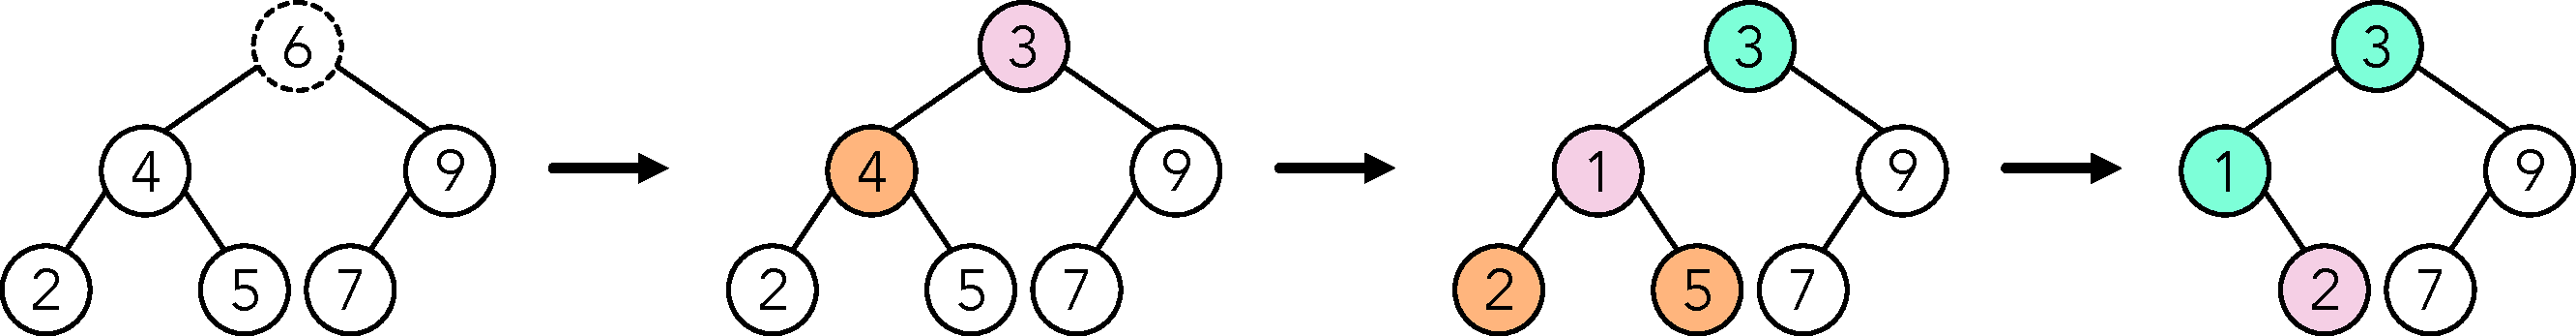
\includegraphics[width=.6\textwidth]{assets/mutate-diagram.pdf}
  \vspace{-2mm}
  \caption{Validity-preserving mutation of a binary search tree, maintaining the
  BST invariant. Mutating the root node from 6 to 3 invalidates the
  4 in the left-hand subtree; the generator 4 with a new random label,
1, then throws away its left subtree (because 1 is the
minimum element of the label range) and relabels 5 to 2.}\label{fig:mutation}
\end{figure}

Between seed extraction and validity-preserving mutation, reflective generators
have the potential to significantly improve on existing tools like Crowbar.

\SUBSECTION{Usability of reflective generators}{sec:reflectiveusable}{3}{3}{HCI
  Practice}{PhD 2}{PhD 4}{Pierce}
Reflective generators are a powerful abstraction, but they are unavoidably a bit
more complex than standard QuickCheck generators. The current design of the
reflective generator language is a best guess at what users will find most
usable (based on our own experience using it) but guessing is far from enough to
ensure usability.

We will evaluate and re-design the surface syntax of reflective generators with
the help of real users.  First, we will recruit a small group of users, teach
them to use reflective generators via a short introductory ``README,'' and ask
them to implement a number of PBT generators inspired by both the research
literature and real-world examples. We will observe the users to identify points
of friction, interviewing them to ensure a clear understanding of their
impressions. With this information in hand, we will identify potential changes
to the API and test those changes with a new group of users. In this way, we
will ensure that both the problems we tackle and the solutions we settle on are
relevant to potential users.

Ultimately, we hope that this process results in a much more usable language for
reflective generators that is simple enough to be used by even non-expert PBT
practitioners.

\SUBSECTION{Generator automation}{sec:genauto}{4}{5}{PL Theory}{PhD 2}{}{Pierce}
%
Even with an ergonomic and learnable language for reflective generators, the
less code the user has to write the better. Our user studies were very clear
that thinking about generators slows users down and makes PBT more challenging.
But we should not compromise: any automation should help users obtain {\em high
quality}, {\em reflective} generators for use throughout the testing process.

As a first step, we will adapt existing tools for type-based generator
automation to work with reflective generators~\cite{noauthor_lysxia_nodate}.
These generators are only useful for testing properties with easily satisfiable
preconditions, but they are a good starting point for many developers. Beyond
that, we consider automation techniques that will help developers interactively
construct reflective generators that maintain complex preconditions.

Some users will have a standard QuickCheck generator that they would like to use
in situations that require a reflective generator. We plan to assist those
users with tools that automatically synthesize the backward annotations
required to make the generator bidirectional. We will experiment with both
conflict-driven program synthesis~\cite{feng_program_2018} or solver-aided
synthesis~\cite{torlak_growing_2013} to see which more successfully generates
annotations for realistic generators. Both approaches have a clearly defined
notion of success: reflective generators have notions of soundness and
completeness that can be tested via PBT, so each candidate set of annotations
can be quickly and efficiently evaluated.

Going one step further, we will also explore techniques that can synthesize an
entire reflective generator from whole cloth. There are a variety of existing
tools that try to do this for standard generators: Lampropoulos et al. provides
two solutions, one based on on inductive relation specifications of
preconditions~\cite{lampropoulos2017generating} and the other based on an
extended language for properties~\cite{beginners-luck}, and Steinh\"ofel et al.
infer a generator from constraints using
Z3~\cite{steinhofel_input_2022,de_moura_z3_2008}. Unfortunately, each of these
tools falls short of solving the problem of automated constrained generation in
general, and none of them include the tools necessary to produce reflective
generators, so there are significant opportunities to advance this space.

\discuss{Do we want to talk about LLMs? This will make Hila and co sad, but we
could do it tastefully...}

\SUBSECTION{Generator benchmark suite}{sec:benchmarks}{1}{2}{Tech
  Transfer}{PhD 2}{PhD 1}{Pierce}
The many papers in the PBT literature demonstrate effectiveness with case
studies, showing that certain bugs in certain systems are caught more quickly
with one tool over another. For theoretical advances, this is often sufficient
to demonstrate that the paper is worth publishing, but this kind of evaluation
can be hard to interpret from the perspective of a would-be user. With all of
the new approaches to generation that we are proposing in this document, and
considering our goals around usability, we need to do better.

We have begun to experiment with a robust empirical evaluation framework for
generators and other PBT techniques. We have built preliminary infrastructure 
for easily and extensibly running experiments to understand testing
effectiveness.  By ``easily,'' we mean that we will take on the burden of
collecting data and analyzing the results, exposing to the user library
functions for their particular instantiations as needed.  When complete, the
evaluation framework will be able to evaluate a given tool based on (1) the
degree to which it is able to achieve high code coverage quickly, and (2) the
speed with which it finds bugs that have been pre-seeded in example programs. By
``extensibly,'' we mean that in addition to the two languages (Haskell and
OCaml/Coq), multiple libraries (QuickCheck, SmallCheck, QuickChick, etc.), and
numerous workloads that we have currently implemented support for, we will design the
infrastructure so that users can easily add new things along each dimension.
Initial observations from this framework have been submitted as an experience
report to ICFP 2023, but many important features (e.g., coverage measurement) have not yet
been implemented.

Our second contribution will codify a library of case-studies and examples as
{\em benchmarks for PBT}. Similar suites of benchmarks already exist in the
fuzzing literature~\cite{hazimeh_magma_2021}, but those benchmarks are not
organized around the particular challenges that PBT tools face. In particular,
few of the benchmarks deal with the kinds of complex preconditions that PBT
tools are built to handle. We want to establish a set of challenging tasks that
can serve as a north star for future improvements to PBT generators and
bug-finding strategies (including our own!).

Initial work and future
designs for this project have been discussed Leonidas
Lampropoulos and his group at the University of Maryland. PI Pierce has a long
history of successful projects with Prof.
Lampropoulos~\cite[etc.]{LuckPOPL,goldstein2021dojudgeatest,lampropoulos_coverage_2019,Lampropoulos&18,OLDlampropoulos19fuzzchick}.

\SECTION{Specification}{Widening the On-Ramp\pagebudget{2}}{sec:spec}
%
\rjmhlater{Notice that the problem of formulating properties is an instance of a
very general problem in automated testing: the 'oracle
problem'. Whenever test cases are generated, rather than hand-written,
the oracle problem arises. You should use those words. Metamorphic
testing was developed specifically as an approach to solving the
oracle problem, and it has a close relationship to PBT. There's a
discussion I think in 'How to Specify it!'.
}
%
To widen the on-ramp to using PBT, developers need help envisioning and writing
specifications. Our pilot study suggested that developers struggle to write
properties about their programs, sometimes due to poorly abstracted code and
other times simply because they fail to see what properties are available to
test. We address the first of these issues in \sectionref{sec:outpurprop} and
the second in \sectionref{sec:interactive}.
%
In \sectionref{sec:automating} we describe a way to automate a
specific high-leverage scenario: model-based testing.
\underconstruction{mention 5.4 too}

\SUBSECTION{Properties over program traces}{sec:outpurprop}{2}{3}{PL
  Practice}{PhD 3}{UGrad/MS 1}{Pierce}
% With current PBT tools, properties can only be expressed over single modules.
% This causes problems when code is organized with functionality crossing module
% boundaries.
A common pain point for developers in our formative research
was that code may not be organized in a way that is conducive to property-based
testing. As a unit testing technology, PBT requires ``units'' of software to
test with clear boundaries. As such, PBT cannot easily apply to programs with
poorly encapsulated global state, or software with leaky or complex abstraction
boundaries.

Could there be a class of PBT tools that supports checking properties of
software in cases where important functionality falls across module boundaries?
We will explore how a PBT tool can support the definition of properties over
cross-module event logs. To demonstrate the potential of such a tool, consider
the case of a developer we interviewed, \participant{7}. P7 was testing
a system, which we call ``\lstinline{Inner},'' exemplifying this messy
abstraction
boundary. It was difficult to test \lstinline{Inner} because
its most interesting behavior arose only when interacting with its calling
component (which we call ``\lstinline{Outer}'').
\lstinline{Outer} took in simple inputs, and used these inputs to construct
complex inputs to \lstinline{Inner}. \lstinline{Inner} could not be tested with
realistic inputs without the complex apparatus of \lstinline{Outer} that
produced those inputs. The developer named this as a circumstance where a
PBT is difficult to apply, because the abstraction boundary between the
components is too fuzzy.

% \TASK{Tools for testing properties over logged values}{2}{2}{Who?}
We will develop a tool that allow developers to express properties that reach
into the state of multiple interacting software components. Take again the
example of \lstinline{Inner}. A solution to P7's problem could be to drive the
test through \lstinline{Outer}, and in doing so implicitly test
\lstinline{Inner}, monitoring runtime values within \lstinline{Inner}. Assuming
\lstinline{Inner} is a routine that processes a stream of messages with internal
values including a queue of processed items \lstinline{processed}, and an
\lstinline{overflow}, properties could include:

\begin{lstlisting}
prefix_of processed (next (processed))       (* 1 Processing is monotonic *)
msg.length < 100 ==> never (overflow = true) (* 2 Can process >= 100 bytes *)
eventually (processed.length = msg.length)   (* 3 whole message processed *)
\end{lstlisting}

Is it possible to check such behaviors with built-in assertion statements? We
posit that an assertion-based approach is non-ideal. On the one hand, assertions
would require nontrivial code to save previous values for properties like (1)
above, and likely involves brittle macros or meta-programming to remove such
auxiliary code at release time. Furthermore, it is difficult to imagine using
the assertion approach to checking properties (2) or (3) at all, because it
would require assertions cognizant of the ``end'' of a computation, information
that may not be available to the assertion statement.

Instead, we propose tooling where properties can be defined over logged values.
The first key component of the tool is the invocation of
logging for specific values using lightweight annotations within modules like
\lstinline{Inner}. The second component is a language for writing temporal
properties over those capable of capturing concepts like \lstinline{next} or
\lstinline{never} from the example properties above. Notably, for such temporal
properties, the property language will require logical connectives not typically
found in PBT. We propose adapting linear temporal logic (LTL) to capture
temporality. We will not be the first to use LTL within PBT; the Quickstrom
framework~\cite{oconnor_quickstrom_2022} uses LTL properties
for specifying and testing graphical user interfaces. That said, considerable
finesse will be needed to adapt LTL to properties at the level of generality
envisioned above; this will be one of the major efforts of the proposed work.

Ultimately, this work will lead to a tool where properties are expressed in a
property language extended with LTL; the system compiles LTL formulae to
properties over log traces; the developer provides inputs to an outer system
\emph{containing} the system(s) of concern; and then the test harness will check
the given trace properties in real time.

\todo{Mention the ``Little Tricky Logics'' paper and say we need to
  consider what logic is really appropriate.}

\SUBSECTION{Mixed-initiative property
  specification}{sec:interactive}{4}{4}{HCI Practice}{PhD 3}{PhD 4}{Pierce}
%
Even when a developer knows when properties are useful in the abstract,
they may still have trouble writing their first properties
for real projects. We plan to develop prototype interactive tools that help
programmers compose their first properties in an educational setting.

The vision of this work is to provide a mixed-initiative~\cite{ref:allen1999mixed}
tool, where a student and their code editor work together to arrive at a
meaningful property. Extending prior work on property extraction techniques (see for
instance~\cite{ref:ammons2002mining, ref:le2018deep, ref:claessen2010quickspec,
smith_discovering_2017}), the idea is to help students compose properties that
are not just accurate descriptors of the system, but significant in reflecting
important program behavior. We will build an interface on top of a property
extractor which helps students write their first properties by allowing them
to (1) identify areas of code likely to lead to adverse behavior;
(2) providing unit test cases that represent special cases of more general
properties; and (3) selecting attributes of data types in the source code, or
of input and output data in a debugging REPL, relevant to the property. These
features will allow a student to more rapidly map from behaviors they can
observe or specify in familiar ways, and see how those behaviors are cast into
the language of their property checker.
%
The tool will be designed for use in Penn's upper division Haskell
course (CIS 5520) and therefore implemented on top of
Haskell's property
generator tool, QuickSpec~\cite{ref:claessen2010quickspec}.

\discuss{Another place to maybe mention LLMs / copilot?}

\SUBSECTION{Model-based properties for
  modules}{sec:automating}{3}{4}{PL Practice}{PhD 3}{UGrad/MS 2}{Pierce}
One finding that has surprised us from the Jane Street study is that
it is {very} common for developers to build (or already to have) a
{\em model
implementation} of the code they are testing and check that the two versions of
the same code produce the same results.  This is a well-documented approach to
PBT~\cite{hughes_experiences_2016}, but it is not supported as well as it could
be by existing tooling.
%
With this in mind, we plan to build comprehensive tooling to automate
model-based testing for systems built in languages with strong {\em
  module systems}, like OCaml~\cite{macqueen_modules_1984}.

Model-based testing is essentially trivial in the simplest case where
the component under test and the model are both pure functions.  But
when the code under test is a {\em
  collection} of functions
organized into a module, things get much more interesting. Testing even a simple
module requires orchestrating multiple calls to the different functions in
its signature. For example, testing the signature \lstinline{StringFns} (in
Figure~\ref{fig:sigs}) requires wiring up the functions in the
signature to satisfy their types: testing \lstinline{drop_n} requires a randomly generated
integer to know how much to drop, calling \lstinline{split} produces a pair of strings
that can each be arguments to future function calls, etc. We will build on prior
work~\cite{hughes_experiences_2016} to generate well-typed sequences of function
calls that can be used to compare module implementations.

\begin{figure}[t]
  \begin{minipage}{.45\textwidth}
\begin{lstlisting}
module StringFns : sig
  val reverse : string -> string
  val drop_n  : int -> string -> string
  val split   : string -> string * string
\end{lstlisting}
  \end{minipage}
  \qquad\qquad
  \begin{minipage}{.45\textwidth}
\begin{lstlisting}
module Set : sig
  type 'a t     val empty : 'a t
  val mem   : 'a t -> 'a -> bool
  val add   : 'a t -> 'a -> 'a t
\end{lstlisting}
  \end{minipage}
  \vspace{-2mm}
  \caption{Some module interfaces we would like to test
    automatically.}\label{fig:sigs}
\end{figure}

Testing modules gets even hairier when they contain {\em abstract types}, as is
the case with \lstinline{Set}. Now some of the types in the signature cannot be
generated on their own, so they must be built up from scratch (in this case by
calling \lstinline{create} and \lstinline{add}). The \lstinline{Set} signature is
also {\em polymorphic}, so a type must be chosen for \lstinline{'a} before
testing. (There is significant work on this
problem~\cite{hou_favonia_logarithm_2022}, but it is not solved in general.)

To solve these problems, we will take a foundational approach, breaking down
modules theoretically and developing automation heuristics from first
principles. This will involve identifying a subset of modules, e.g., potentially
those that use generation-unfriendly types like GADTs, where automation is {\em
not} possible; highlighting that subset will provide useful context for future
work that might aim to simplify these cases in other ways (e.g., by putting a
human in the loop).

The work in this project will ultimately provide a recipe for automating a
significant swath of testing situations, massively lowering the barrier to entry
for PBT in ML-based languages. It will also provide a basis that others can
build on in other languages: abstract and polymorphic signatures are features of
many other modularity mechanisms (e.g., Java interfaces, Rust traits, Haskell
type classes, etc.), so solutions we find in OCaml should transfer.

\iflater
\bcp{I wonder whether one of the attractions of model-based properties for real-world testing is that they more or less allow one to ignore the issue of "generating structures satisfying preconditions."  That is, if what you're doing to build an "interesting" value of some data structure or internal state of some stateful system is issuing calls through an API, then I would guess in most situations pretty much any sequence of API calls will be legal; some will be more interesting than others, of course, but at least you'll never build a structure that doesn't satisfy the preconditions of your operations -- your whole distribution will always fall within the space of well-formed structures.  (Or, if it observably doesn't, you'll have uncovered a bug.)
Could this help explain why it seems to be so prevalent, at least at
Jane Street?  Is there any way one could test whether this sort of
reasoning is an actual explanation for the observed prevalence?  Is
any of this worth mentioning here?}
\hg{We keep conflating ``model-based'' testing (test against an oracle
implementation) with ``state-machine'' testing (test by calling a stateful API
over and over).  It's understandable, since a lot of state-machine testing is
model-based, but my recollection is that our observations of JS developers
actually leans toward model-based testing that {\em isn't} state-machine
testing. That's a thing we should remember to double check for the full
analysis. But in any case, I think model-based tests are easier to think about
even when generating inputs from scratch, because you don't have to think about
logical properties. Not sure if there's any way to squeeze this discussion in,
or if we should}
\fi

\SUBSECTION{Automatic explanations for properties}{sec:understanding}{4}{5}{HCI
  Theory}{PhD 3}{}{Pierce}
%
As is often the case for code of any kind, the specification of a property may
not be self-explanatory. This is particularly the case when those properties are
found by programmers who did not write them, and can be exacerbated if the those
programmers have never used property-based testing themselves. Can we design
tools that help programmers understand property specifications?

We envision several approaches, drawing inspiration from recent HCI research.
Prior work has demonstrated the potential of generating meaningful explanations
for simple programs, whether those explanations are consist of text
explanations~\cite{ref:head2015tutorons,ref:mayer2015user},
visualizations~\cite{ref:guo2013online}, or
counterexamples~\cite{ref:dantoni2015can}. These techniques tend to work when
programs are short in length, draw mostly from simple syntax, and are
structurally simple.  While properties can be rather long, they are often
comprised of relatively simple language idioms (i.e., a number of function
calls, conjunctions, and implications). For this reason, it may be that these
ideas could generalize to helping newcomers to properties understand those
properties well enough to understand them generally, and perhaps even make
lightweight modifications, without needing to seek out dedicated instruction for
the PBT framework.

The first sort of explanation we will provide is at the level of explaining
syntax, similar to that proposed for Unix commands~\cite{ref:head2015tutorons},
synthesized programs~\cite{ref:mayer2015user}, and Hazel
code~\cite{ref:potter2022contextualized} in prior work. Commonly, PBT frameworks
require the use of a custom property language. This is the case, for instance,
for Haskell's QuickCheck. For users who are familiar with the host language but
not the property language, we will design tooltip explanations that explain
particular idiomatic constructs including symbols and common structures in
property-based tests. Our efforts will focus on understanding the language with
which to describe properties to those unfamiliar with property-based testing,
and to identify those syntactic anchors in the code that are sensible sites for
programmers to access automatic explanations.

The second sort of explanations will be examples, namely, sampled input-output
pairs that can convey the behavior of the program with respect to the property.
The advantage of example-based explanations is that a solution to this problem
for one PBT framework may generalize to others; while not all frameworks use
special property syntax (e.g., Hypothesis), all frameworks have the potential to
have rather long properties. Some of the simplest (perhaps smallest) passing
inputs will be selected as example inputs. These examples will be perturbed to
generate similar negative examples. Example pairs will be shown alongside the
code in the editor using editor annotations. This project will dovetail with our
project on interactive debugging (\sectionref{sec:failures}) to identify
test cases that are likely to best ``explain'' intended program behavior.

Given recent trends in computing research, it bears mention that large language
models such as GPT3 may merit consideration for generating descriptions of the
high-level ``idea'' behind properties; PI Head is investigating similar ideas
for understanding generated code in general purpose programming languages. While
we intend to explore this to some limited extent, most of our efforts will be
spent on the two approaches above involving rule- and example-based
explanations, given their applicability to property languages for which there
may not yet have been data incorporated into modern large language models.

\iflater\todo{Tweak the title when we understand the content. :-)}\fi

\SECTION{Interaction}{PBT at Users' Fingertips
 \pagebudget{3}}{sec:val}

In this section, we
describe a sequence of research efforts to design and evaluate usable developer
tooling for PBT. These projects will contribute new paradigms for assessing whether their generators are generating sufficient and
appropriate inputs (\sectionref{sec:evaluating_distributions}) and whether those
inputs sufficiently exercise their code (\sectionref{sec:tuning}),
and understand testing-provoked failures involving complex inputs
(\sectionref{sec:failures}).
%
In \sectionref{sec:counter} we describe a planned tool to help migrate
counterexamples found by property-based tests into conventional
regression tests.
%
These projects will all be pursued using HCI
methodology, integrating these tools into contemporary interactive development
environments. The success of tools will be evaluated in usability studies
comparing developers' effectiveness and efficiency in writing tests for their
software, and debugging problems discovered by their test suites.  PI Head will
guide tool development efforts, leveraging his
experience designing, developing, evaluating, and deploying novel programming
environments and
tools~\cite{ref:head2015tutorons,ref:suzuki2017tracediff,ref:head2017writing,ref:head2018when,ref:head2018interactive,ref:head2019managing,ref:head2020composing}.

\SUBSECTION{Evaluating data
  distributions}{sec:evaluating_distributions}{2}{3}{HCI
  Practice}{PhD 4}{UGrad/MS 3}{Head}
%
In comparison to testing techniques like unit testing, PBT draws many
tests from some
random {\em distribution} over possible inputs, rather than writing down a few
concrete individual inputs. The success  of
PBT thus depends on the quality of this distribution---whether
most of its probability mass is on tests that are sufficiently
realistic and diverse. We plan
to develop tooling for
understanding distributions of input data and easily tuning them.

\begin{wrapfigure}{r}{0.58\textwidth}
  \centering
  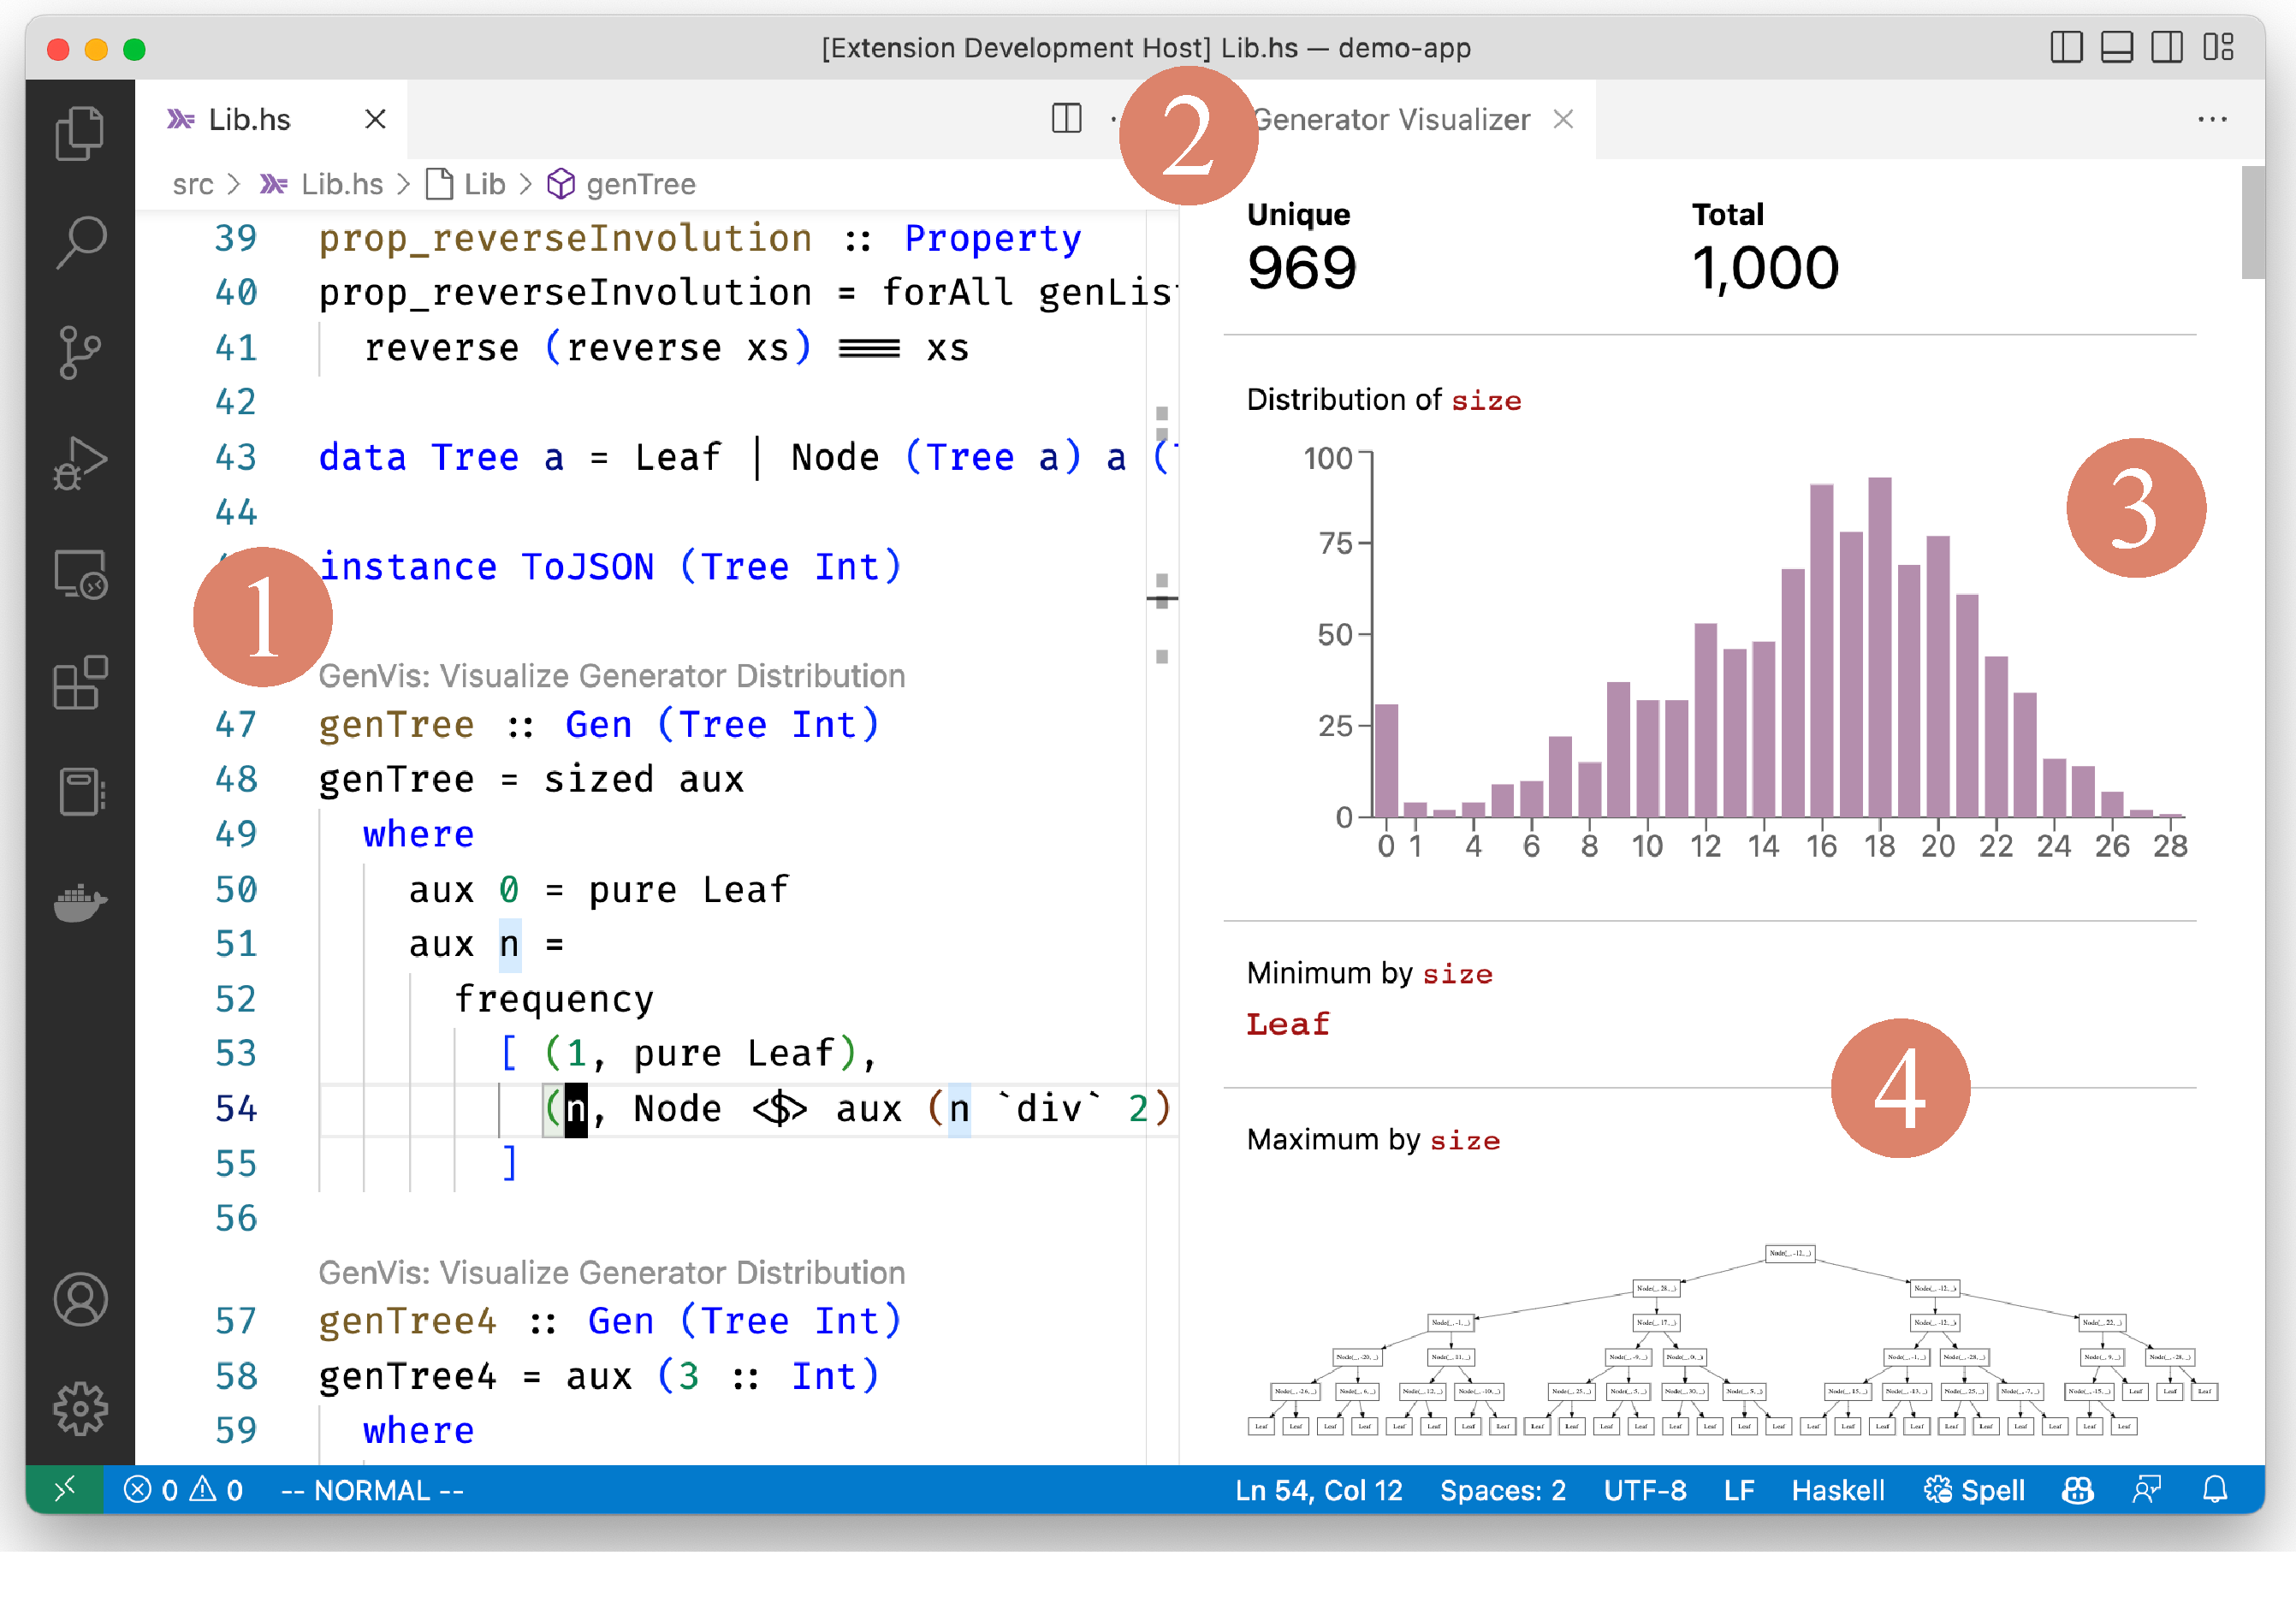
\includegraphics[width=0.58\textwidth]{assets/gen-vis.pdf}
  \caption{An envisioned tool for evaluating data distributions.
    \todolast{put this near the text that refers to it}}\label{fig:gen-vis}
\end{wrapfigure}

We draw inspiration from related work in HCI that has sought to better expose
the shape of input data distributions including
machine learning datasets
(e.g.,~\cite{ref:hohman2019gamut} and
~\cite{ref:hohman2020understanding}) and sequences of program values
(e.g.,~\cite{ref:kang2017omnicode}).
PBT poses a unique challenge because test inputs are
programmatically generated and
can be of unbounded structural
complexity (e.g., lists, trees, and other algebraic data types,
sequences of API calls, ...).
Consider an
example from a participant in our formative study, who wanted to generate
realistic logs of input data, where each log entry included at least a timestamp
and an event type.
% \proposecut{Such values are not trivially plotted in conventional
% visualizations, and it would be prohibitive to review individual examples if the
% logs are sufficiently long.}
Ideally, a developer would be able to answer
questions like: Are the generated log inputs long enough? Are the
event sequences
realistic? This setting requires new kinds of views of data and tight
developer support for easily defining meaningful views of the data.

% \TASK{Tools for working with data distributions}{2}{3}{who?}
We will design and implement new interactive tools that provide rapid,
informative views of input data distributions. The tools will address the
challenges of visualizing generator distributions using a novel combination of
tailored, tried-and-true features for interactive programming environments.

First, our tools will support live, realtime displays of generated values.
Our first goal is to provide
instant, live~\cite{ref:tanimoto1990viva} feedback on the generators. Building
on the tradition of other live functional programming environments
(e.g.,~\cite{tool:lighttable,ref:omar2019live}),
% our environment will provide
% live feedback summarizing many inputs produced by a generator, rather
% than a single one; As testing proceeds,
our environment will sample inputs
output by the generator and
pipe them into data displays (Figure~\ref{fig:gen-vis}), which
will first and foremost show aggregate data views, including aggregate
statistics (Figure~\ref{fig:gen-vis}.2) and visualizations of the distribution
of key features of the data (Figure~\ref{fig:gen-vis}.3). Visualizations will be
generated according to simple recommendation rules, similarly to other recent
exploratory data visualization tools from
HCI~\cite{ref:lee2021lux,wongsuphasawat_voyager_2016,
wongsuphasawat_voyager_2017}. Unique to our project, features to visualize will
be based on awareness of common features of algebraic data types, and extensible
through lightweight user-written code. For example, consider the
\lstinline{log} type
described above. A developer might be interested in the log's
\lstinline{length}, field accessors like \lstinline{event_type}, \lstinline{id},
and \lstinline{timestamp}, filters like \lstinline{is_empty}, and even
aggregators like \lstinline{max_by}. These kinds of features can be
generated automatically for common data types.
% Then the tool will then use
% lightweight type-based program synthesis to compose and combine these functions
% to get features. It may choose to show the \lstinline{length} of a log, but also
% the \lstinline{max_by (fun l -> length l.payload)} (the maximum payload length),
% and even pairs of features like these (which could be viewed as a two
% dimensional feature).

Second, the data displays will be easily extensible, via lightweight customization hooks. If
there are features that the user notices should be extracted, but that the
system cannot come up with itself (e.g., \lstinline{ids_unique}) the user can
write it themselves in companion code alongside their property specifications;
the interface will automatically load those features into the display.

Third, the interface will make it possible to drill down into
individual inputs from a list of samples that can be
filtered by selecting marked visualizations (e.g., choose a bar
of length ``10'' to preview individual inputs with that length). One
challenge will be to provide suitable representations of complex inputs that
will be easy to understand. Some general solutions might be to
pretty-print inputs, provide interactive object browsers like those available
in JetBrains~\cite{tool:jetbrains}, and/or allow a developer to explore an
object using a built-in REPL. Additionally, we will produce DOT
graph~\cite{ellson_graphviz_2002} representations of common kinds of inputs
(i.e., lists, trees) that will provide an at-a-glance understanding of
larger inputs (Figure~\ref{fig:gen-vis}.4).

Finally, our tools will provide live feedback on the input
distribution in the form of in-situ coverage feedback. Like other HCI
prototypes that have shown which lines of code are currently
executing in a running program~\cite{ref:brandt2010rehearse,
  ref:oney2009firecrystal, ref:burg2013record}, ours will be
able colorize code in the editor on the basis of
how frequently each line has been executed while running tests.

The result of these experiments will be the first live tool for generator
feedback and analysis; in the next section, we take it one step
farther to consider how interactive tools can help a developer not
just understand input data distributions, but more directly change
them.

\SUBSECTION{Tuning data distributions}{sec:tuning}{3}{4}{HCI
  Practice}{PhD 4}{UGrad/MS 4}{Head}
%
Tuning generator distributions is a challenging task, often requiring
significant trial-and-error---changing generator parameters and hoping
that the input data distribution changes in the right way. Approaches
like the one in \sectionref{sec:reflective} can help, but manual tuning
is still needed in many cases.
Developers need higher-level ways to describe the kinds of inputs they.

We will design tools to support the direct tuning of input data distributions
through manipulation of generated inputs and data distribution
visualizations. This work will build on the foundation outlined in
\sectionref{sec:evaluating_distributions}. Inspired by recent tools in
the PL+HCI literature
for bidirectional manipulation of programs and their
outputs~\cite{ref:hempel2019sketch, ref:kery2020mage,
  ref:omar2012active, ref:omar2021filling},
we explore reflective generators' potential to support tuning.

% \TASK{Tuning by filtering}{3}{4}{who?}
First, a general method for tuning input data distributions will be to
define filters on input data by manipulating aggregate data displays.
For instance, developers will be able to select a range of values from a bar
chart showing input data features and then request that all values generated
within that range are discarded before testing. This approach is flexible,
though it is notably coarse-grained;
it does not influence the implementation of the underlying generator, and
therefore can only go so far in influencing the kinds of values that are
generated.

% \TASK{Tuning by reflection}{3}{4}{who?}
A second idea is to leverage
reflective generators (\sectionref{sec:reflective}) to change the underlying
generator parameters. Developers will be able to interact with a visualization,
and then the the reflective generator will map those interactions
back to choices
in the generator (e.g., what value to place in a node, or the number of nodes to
produce, etc.), which can then be made more or less frequently. We envision
building tools that show the generator code
side-by-side with visualizations, and where parameter choices in the generator
can update live as the data distribution is manipulated in the visualizations.
Furthermore, developers will be able to interact with individual data points,
expressing that they would like to see more inputs like one that has already
been generated, or that they would like an input similar to a generated input,
but different in a way that they have demonstrated. Together, this tool and the
tool for visualizing generated data distributions will have a synergistic effect
in improving developers' ability to understand and ultimately achieve more
realistic, comprehensive data distributions for their testing.


\SUBSECTION{Interactive shrinking and
  debugging}{sec:failures}{4}{4}{HCI Practice}{PhD 4}{PhD 2}{Head}
%
One of the challenges in using PBT is understanding why
a given counterexample triggers a bug.  We will design interactive
tools to help in this process.

First, we will design tools that build on
shrinkers~\cite{hughes_quickcheck_2007,arts_shrinking_2014} to help developers
understand counterexamples. Automatic shrinking, even when done via reflective
shrinkers as we discuss in \sectionref{sec:reflective}, can be opaque, and
shrinkers can get stuck at local minima that far from the global minimum.
But developers can often see shrinking options that the shrinker does not know to consider.
Drawing inspiration from approaches in recent HCI literature that support
interactive code reduction through iterative, incremental
experimentation~\cite{ref:lim2018ply,ref:head2018interactive,ref:holmes2012systematizing,ref:hibschman2016telescope},
we will design aids for rapid, incremental, interactive shrinking of complex
inputs into simpler inputs. The key feature we will develop is the ability to
shrink inputs semi-automatically by manipulating the input's contents and structure in an interactive
object viewer, similar to the kinds of object viewers available in contemporary
debuggers like in the JetBrains IDE~\cite{tool:jetbrains}.

The interactive shrinker may display the valid in which an input can be pruned,
relying on reflective generators to provide the insights into which parts of the
structure correspond to valid changes. Alternatively, the developer might change
the input entirely, for example, noticing some change of inter-dependent parts
of the structure that shrinking missed.  As a developer manipulates the input,
automatic shrinking will continuously be re-tried, reducing the input further
and giving feedback as to whether it still causes a test to fail or not.
Developers will ultimately be able to reduce complex counterexamples into
simpler ones that are easier to reason about when looking for bugs.

In addition to developing novel interaction techniques for simplifying inputs,
we will also develop systems for helping developers locate code that, if
changed, would resolve the failure. Rather than explicitly encoding
relationships between generated outputs and their dependencies on
code~\cite{ref:ko2009finding}, we will instead help the developer
understand where the execution paths of a given counterexample diverges from
successful yet very similar inputs.
\hg{Zac says: Hypothesis has this in the “explain” phase, which will be enabled
by default later this year.  Debugger integration sounds neat, though what I'd
really love to see would be integration with an rr-style time-travelling
debugger - annotate the minimal trace with information from other traces!  For
example, using static and dynamic slicing to show the user where (and what) in
the trace is responsible for failure… -- @Andrew what do you think?}
Leveraging the parametric nature of the
reflective generators, we will generate inputs in a space ``around'' a
counterexample and identify which ones no longer cause a failure.  Then, we will
execute the program up to the point where the traces of the programs begin to
diverge, and we will drop the programmer into a debugging environment where
they can query the state of the program and step through the remainder of the
execution. PI Head has prior work designing debugging tools that help
programmers understand trace divergences in an educational
settings~\cite{ref:suzuki2017tracediff}; the work of this project would be to
bring this technology into professional programming environments where traces
for similar inputs are abundant.

% \iflater
% \SUBSECTION{Dashboards for long-running
%   tests}{sec:dashboards}{4}{5}{Tech Transfer}{PhD 4}{Engineer}{Head}
% %
% \discuss{Harry and Benjamin wonder whether this section can be
%   dropped.  It seems (a) smaller than the other tasks and (b) maybe
%   less interesting in the grand scheme?  (We can still do it, and
%   indeed we can mention it in the \tyche{} section, but not give it a
%   whole top-level section.)  We are also a bit past the limit of how
%   many tasks is plausible.}

% \underconstruction{ \iflater\todo{Write me Andrew?}\fi
% \begin{itemize}
%   \item Given the random nature of tests, it is not guaranteed that the same
%     software, when tested twice, will have the same results.
%   \item Views that focus on specific, known test cases may then be easier for
%     developers to understand quickly than those reporting summary statistics.
%   \item Or, dashboards should bring together signals from both random samples
%     of inputs, as well as known samples.
% \end{itemize}
% }
% \iflater \hg{I copied a comment into here---can we use any of that writing for this
% section?}\fi
% \fi

% \ifdraft
% \SUBSECTION{Increasing Assurance with More Tests}{sec:more}{3}{4}{Andrew}{}{}

% The informants in our interview study admitted to heuristic
% approaches to determining how many tests to run. Many set
% rigid cutoffs such as one-thousand tests, or one minute's
% worth of tests. One reason for these heuristics was that
% developers did not want to lock up their computer's
% computational resources, or delay their other development
% tasks, by waiting for their property-based tests to
% complete. As one of our informants pointed out, this could
% lead to circumstances where bugs were not discovered until
% property-based tests were checked into the continuous
% integration system, when tests were finally conducted at a
% sufficient volume to generate failing inputs \amh{@HG can
% you fact check my paraphrase of this informant's input?}\hg{Technically this was
% a pilot study informant, but I think it's OK}.
% Unfortunately, when failures are detected in continuous
% integration, developers no longer have the context to
% address those problems easily, because they have likely
% moved on to other tasks.

% We believe that, if appropriately designed, a developer's
% PBT tools can help developers get the best of both
% world: they can both increase assurance that their software
% is correct by running more property-based tests, while not
% locking up their computer's resources. We propose to extend
% in-editor testing tools to permit options where developers
% can configure their PBT test drivers to continue testing
% software in the background by default, without requiring a
% developer's explicit input. These tools will scan a
% developer's environment for property-based tests, divide
% time proportionally between the various tests, and capture
% the results in a digested form. To reduce the likelihood of
% breaking a developer's focus, errors will be marked through
% subtle annotations in the code (e.g., icons in the line
% margins) when one has been detected. Developers can also
% request alerts that can report failures instantaneously,
% should they wish to address any discovered failures right
% away.

% \hg{This section needs honing; right now it's just what I wrote in my thesis
% proposal, and it's too high-level} \amh{Is this a user
% interface project devoted to figuring out ways of invoking
% and keeping tabs on long-running tests during solo
% programming? Or is it a project around proposing better
% software engineering process that gives the right amount of
% time to long-running PBT tests?}
% \hg{Good question. I kind of naively hoped it was a UI project that both helped
% users invoke and keep tabs of tests in the background AND pushed them towards
% software engineering processes that gave PBTs appropriate space to operate. But
% now that I think about it that seems like a lot at once. Honestly I think the
% cultural shift in SE (potentially backed by some large-scale software tools) is
% the more impactful angle, but I don't know if we can argue that we know how to /
% want to do that}
% \bcp{Delete the section?}
% \amh{I tried this section again, trying to spell out in more
% detail my updated conception about what would be useful and
% magical about this tool. Can someone else take a look at it
% and make the decision of whether to remove the section?}
% \hg{I think it's better, but it's still pretty vague and flat. I wish there was
% a specific example of an interaction that I could say ``oh yeah, why don't I
% have that?'' As written, it sort of feels like the devil is in the details and
% we didn't actually give an details}

% % It is likely that PBT tools could play a role in improving this state of
% % affairs. For example, one could take inspiration from some theorem
% % provers~\cite{berghofer2004random} and create a system in which properties are
% % checked locally but in the background, as the programmer works on other things.
% % This avoids waiting time while potentially being less frustrating than running
% % in CI, since bugs would likely be found while the programmer still had the code
% % ``paged in.'' Alternatively, one might design a PBT system with CI in mind,
% % providing automated features for deferring property failure notifications until
% % a specified time or turning failing properties into unit tests that can be saved
% % for future testing.

% \fi

\SUBSECTION{Counterexamples as regression
  tests}{sec:counter}{5}{5}{HCI/PL Practice}{PhD 4}{}{Head}
%
% After testing has revealed a counterexample to one of their properties
% with their tests, the developer may wish to turn that failure into a
% regression test, to ensure that later
% changes to the code will not reintroduce the same failure.
One pain
point experienced
by informants in our interviews at Jane Street was that it requires considerable work to
transform a failure that was detected by their PBT tools into a
regression test, despite the fact that much of the work involved in doing so
felt mechanical.

% \TASK{A tool for turning counterexamples into tests}{2}{2}{who?}
We plan to develop usable tooling for transforming failed PBT tests into single
regression tests. What is important to note about this project is that creation
of regression tests is \emph{mostly}, but not entirely, mechanical. In reality,
the creation of regression tests will likely require judicious incorporation of
the developer's input at key decision points. This is particularly the case for
specifying acceptance criteria. For instance, consider a property that checks
that a list insertion function never produces an empty list. In the event of a
failure, a developer may want to produce a regression test checking the
exactness of the result on the failed input (e.g., checking that the insertion
produced a particular concrete list) rather than simply checking that the output
list is non-empty.  Writing a regression test may involve multiple such
choices, including whether to test for exact output, whether to test
intermediate results, and how to initialize inputs.

We will develop an interactive tool that assists developers in creating
regression tests from failed tests. The idea is to first develop
technology for generating sufficiently readable code for regression tests (using
approaches such as Daka et al.'s~\cite{ref:daka2015modeling}), and then provide
in-situ editing assistance along the lines of contemporary interactive
refactoring tools from the HCI
literature~\cite{ref:head2018interactive,ref:barik2016quick,ref:murphyhill2008refactoring,ref:lee2013draganddrop}.
For this unique task of transforming properties into regression tests,
our tool will \iflater\proposecut{provide the key features
  of}\hg{MINOR: Feel free to disagree,
but I think phrases like this are a bit of an anti-pattern. I'd rather just say
the tool will X}\fi keeping track of the failed input,
generating starter test code, substituting in correct expected values of the
output by executing corrected code, and supporting developers in rapidly
performing likely edits to regression tests by providing suggestions of
alterations to their code like the ability to generate general property checks
with precise equality checks\iflater\bcp{??}\hg{I also don't understand what this is
getting at}\fi. We also hope the results of this work
can inform the
design of other approaches to counterexample extraction, including one that is
proposed for the Hypothesis library in Python~\cite{maciver2019hypothesis}.

\SECTION{Diffusion}{Advancing Open Source PBT Tooling}{sec:diffusion}

\forreaders{This section collects all the tasks that involve either
  primarily engineering or primarily education.}

\underconstruction{Needs an introduction.}
%
A notable finding of the Jane Street study has been that widening the
on-ramp to PBT may be easier if we can point developers towards particularly
high-leverage use-cases for PBT. In \sectionref{sec:whento} we discuss our plans
to catalog and communicate these use-cases for developers.

% \bcp{If we're going to keep this as a top-level theme, we'll need to
%   integrate it into the motivation early on (i.e., give it a color,
%   talk about how the Jane Street study shows we need it, ...).  Many
%   of the specific items fit just fine into the sections we've got (and
%   I moved them there).  But I wonder whether a top level ``Diffusion''
%   or ``Integration'' theme might be helpful for the story, and as a
%   catch-all for the rest.  Thoughts?}

% \hg{I think I like the idea of a section where we can talk about what the
% engineer will do without having to shoehorn it into others' projects. E.g., the
% engineer will theoretically be making changes to Hypothesis based on findings
% from Jane Street, reflectives, etc. but it's hard to talk about open-source
% maintainence in those sections. It will be difficult to justify diffusion based
% on the JS study, but it'll be a no-brainer if we justify it from the perspective
% of the ``grand challenge'' of establishing a cohesive, multi-language ecosystem
% for usable PBT}\bcp{Yes.  I think as we reshape and scale up the
% overall structure, we need to move away from the JS study as providing
% the whole architecture for the proposal: it was a nice conceit for a
% smaller project, but this one reaches too far beyond.  The grand
% challenge is better motivation for the whole thing.}

\SUBSECTION{Beyond research software}{sec:engineersupport}{3}{5}{Tech
Transfer}{Engineer}{}{Pierce}
%
The research projects we have proposed thus far will have the potential to
dramatically improve the power and usability of PBT systems, but only if those
systems are attractive to real users. There is an unfortunate tendency for
research software to remain ``research software,'' missing critical
documentation that new users need to get started and lacking a clear
maintenance schedule that would give software companies the confidence to adopt.
To avoid this fate for our projects, PhD students will work closely with our
research engineer. Projects will be designed with learnability and
maintainability in mind, and upon completion they will be handed off to the
engineer to grow and maintain.

Concretely, we expect the research engineer to be involved in the following
projects:
\todo{Add titles}
\begin{itemize}[noitemsep]
  \item \sectionref{sec:frameworks}: Helping PhD 1 to build and maintain a minimal PBT
  framework for use in comparison studies.
  \item \sectionref{sec:reflective}: Implementing and maintaining versions of
  reflective generators in a number of languages and PBT ecosystems, with the
  help of PhD 2.
  \item \sectionref{sec:interactive}, \sectionref{sec:counter}: Assisting PhD
  3 with maintenance of tools for easier property specification.
\end{itemize}
Most importantly, the research engineer will help to build and maintain
\tyche{}, the IDE for PBT designed as part of PhD 4's dissertation. We
describe this effort in more detail in the next section.

\SUBSECTION{Tyche: An IDE for PBT}{sec:ide}{2}{5}{Tech
  Transfer}{Engineer}{PhD 4}{Pierce}
The projects in \sectionref{sec:val} design a wealth of new modes of interaction
for PBT. These interactions will be valuable for developers on their own, but
their impact can be significantly magnified if they are integrated together in a
place that is easily accessible to would-be users. This is the inspiration for
\tyche{}, an integrated development environment (IDE) for PBT.

\tyche{} will include all of the functionality designed in \sectionref{sec:val},
including tools that facilitate more intentional PBT workflows, interact with
and improve the programmer's generator code, and assist in the test-authoring
and debugging processes---all integrated into Visual Studio Code, a popular
and extensible programming environment.
While \tyche{} is going to be language-agnostic where possible, the Hypothesis
developers have even recommended that we try to include a Python-optimized fork of
\tyche{} into the main Python language extension.

The research engineer will assist in the integration process, ensuring that the
extension is more than the sum of its parts. Indeed, we plan for \tyche{} to
live on as a home for further innovation: future tools that we or others in the
community see as important improvements to PBT workflow will also be included
over time.  With a strong theoretical grounding and consistent engineering
support, \tyche{} will provide an efficient pipeline for bringing research on
PBT interaction models to software developers craving better tools.

\SUBSECTION{Nurturing the PBT ecosystem}{sec:nurturing}{1}{5}{Tech
Transfer}{Engineer}{PhD 1}{Pierce}
The ecosystem of existing open-source PBT tooling is broad and varied. Some
projects are vibrant and well-maintained, while others, including some with
great ideas and implementations, do not have the developer bandwidth to address
user needs. Additionally, different libraries for PBT vary wildly in their
ideological approaches, as we outline in \sectionref{sec:frameworks}, making
skill transfer difficult for users. For these reasons, we will allocate
engineering time focused on supporting and improving open-source libraries for
PBT.

To address the problem of under-maintained software projects, we will simply
reach out to the maintainers of projects with important outstanding issues and
ask the maintainers (if any exist) what help they need. We are already in
contact with Zac Hatfield-Dodds, the main maintainer of Hypothesis, and he has a
variety of library improvements that could benefit from more developer support.
Other projects, such as Crowbar in OCaml, various smaller generator libraries in
Haskell, and the PBT frameworks in Rust seem like high-value libraries worth
assisting.\hg{Not sure how best to frame this. Maybe the answer is just less
detail...}

There are two ways we may be able to help solve the problem of skill transfer
between PBT libraries. Where possible, we hope that the project from
\sectionref{sec:frameworks} provides us with enough evidence to convince some
library designers to take a different tack and make their library more like
others. In that case, we will provide engineering support to ease that
transition. In other cases, where both approaches have benefits, we will
generate documentation that helps developers move from one library to another.

On the topic of documentation: the PBT ecosystem, like every software ecosystem,
is woefully under-documented. If the research engineer on our team is ever
waiting for work, they will also help to improve the state of documentation for
high-value PBT libraries.

These activities will all contribute to a more cohesive and consistent PBT
ecosystem, making PBT an easier choice for both companies and individual
developers.

\SUBSECTION{``When to Specify
  It!''}{sec:whento}{1}{1}{Education}{Faculty}{Everyone else}{}
%
\todo{Transition}
Our first pilot study with users of PBT suggested that developers struggle to
come up with specifications that are worth
testing~\cite{goldstein_problems_2022},
but
our follow-up interviews at Jane Street suggest that the developers there
rarely have the same problem. It seems that the Jane Street developers had
a tacit
understanding of ``no-brainer'' situations where PBT was an obvious
choice---situations where properties were easy to find and where PBT provided
much more thorough testing than other common techniques---and they limited their
use of PBT to these situations.
While experienced PBT users do also apply it in
high-cost / high-benefit situations, we believe
focusing on easier cases is the best way to drive adoption.

We aim to produce authoritative resources that help developers understand
high-leverage situations for PBT. We will begin with an effort
tailored to the academic community: a survey paper with the
aspirational title ``When to Specify It!'' in homage to John Hughes'
widely-viewed tutorial ``How to Specify It!''. This survey will
document the range of high-leverage scenarios identified in our formative
research, including cases like
\begin{enumerate*}[label=(\arabic{enumi})]
\item ``these two functions (e.g., a parser and a printer) should round-trip,''
\item ``this data structure (e.g. a set, map, etc.) should obey algebraic laws,''
\item ``this stateful module should uphold an invariant,''
\item ``these two programs should behave the same'' (e.g., because one
is an optimized version of the other),
and
\item ``this program should not crash.''
\end{enumerate*}
This list will be further expanded with our follow-up surveys with broader
communities of developers~(\sectionref{sec:survey}), a comprehensive
review of case studies that appear in
the academic literature, and an examination of open source projects across a
variety of different software ecosystems using PBT (e.g.,
QuickCheck/Haskell, Hypothesis/Python, Quickcheck/OCaml).

Building on the strong foundation of the survey, we will distill our findings
into media directly tailored for developers. First, we will write up
approachable developer documentation in partnership with our industry
collaborators, to be read among the first resources of any developer
documentation on PBT tools. We will work with our industry collaborators to
disseminate this documentation in blogs and incorporate it into tool
manuals. Then we will package the findings as a talk for one or more
professional developer conferences.

\SUBSECTION{PBT for
  undergraduates}{sec:1210}{1}{5}{Education}{Faculty}{Engineer}{}
\iflater\bcp{Should this be led by BCP, or both?  Say explicitly.}\fi
\todo{Transition}
%
Education can act as a force multiplier to make technologies more usable.
When tools or techniques become standards in undergraduate curricula,
students help bootstrap adoption of those tools and techniques in industry. We will
integrate PBT into some of the earliest coursework that undergraduate students
take, targeting introductory level data structures
curriculum. As noted in \sectionref{sec:whento}, testing well-defined data
abstractions is one of the high-leverage scenarios for using PBT, making data
structures a powerful anchor for demonstrating the power of PBT. Building on the
foundation of recent PBT instruction in data structures
courses~\cite{wrenn2021using,nelson2021automated}, we will integrate PBT into
Penn's CIS 1210 course on data structures. We
will evolve the curriculum to emphasize themes in PBT that have arisen from our
formative research to help students identify powerful circumstances for
using PBT, including methods for writing great generators, understanding
generators, considering properties as documentation, and expanding one's
thinking around the scenarios where PBT is suitable
(see~\sectionref{sec:whento}). We will evaluate the impact of these new
instructional approaches on students' ability to leverage PBT in final projects,
disseminating our findings in publications at computer science research venues.
The instructional materials we develop will be made public for instructors at
other institutions to adapt into their own curricula.

\amh{Add evaluation of new contributions to the curriculum, with plans to
publish findings in computing education research venues.}

\immediate\closeout\workplanfile
% \SIMPLESECTION{Plan of Work\pagebudget{.7}}{sec:plan-of-work}

% \bcp{I've moved the text that was here to a separate supplemental
%   document, but we'll probably want to say something short in the main
%   project description (either here or, better, toward the top) about
%   synergy and coordination, with a pointer to that document.}

% \begin{figure}[ht]
%   \centering
%   \vspace*{-1in}
%   \hspace*{-.4in}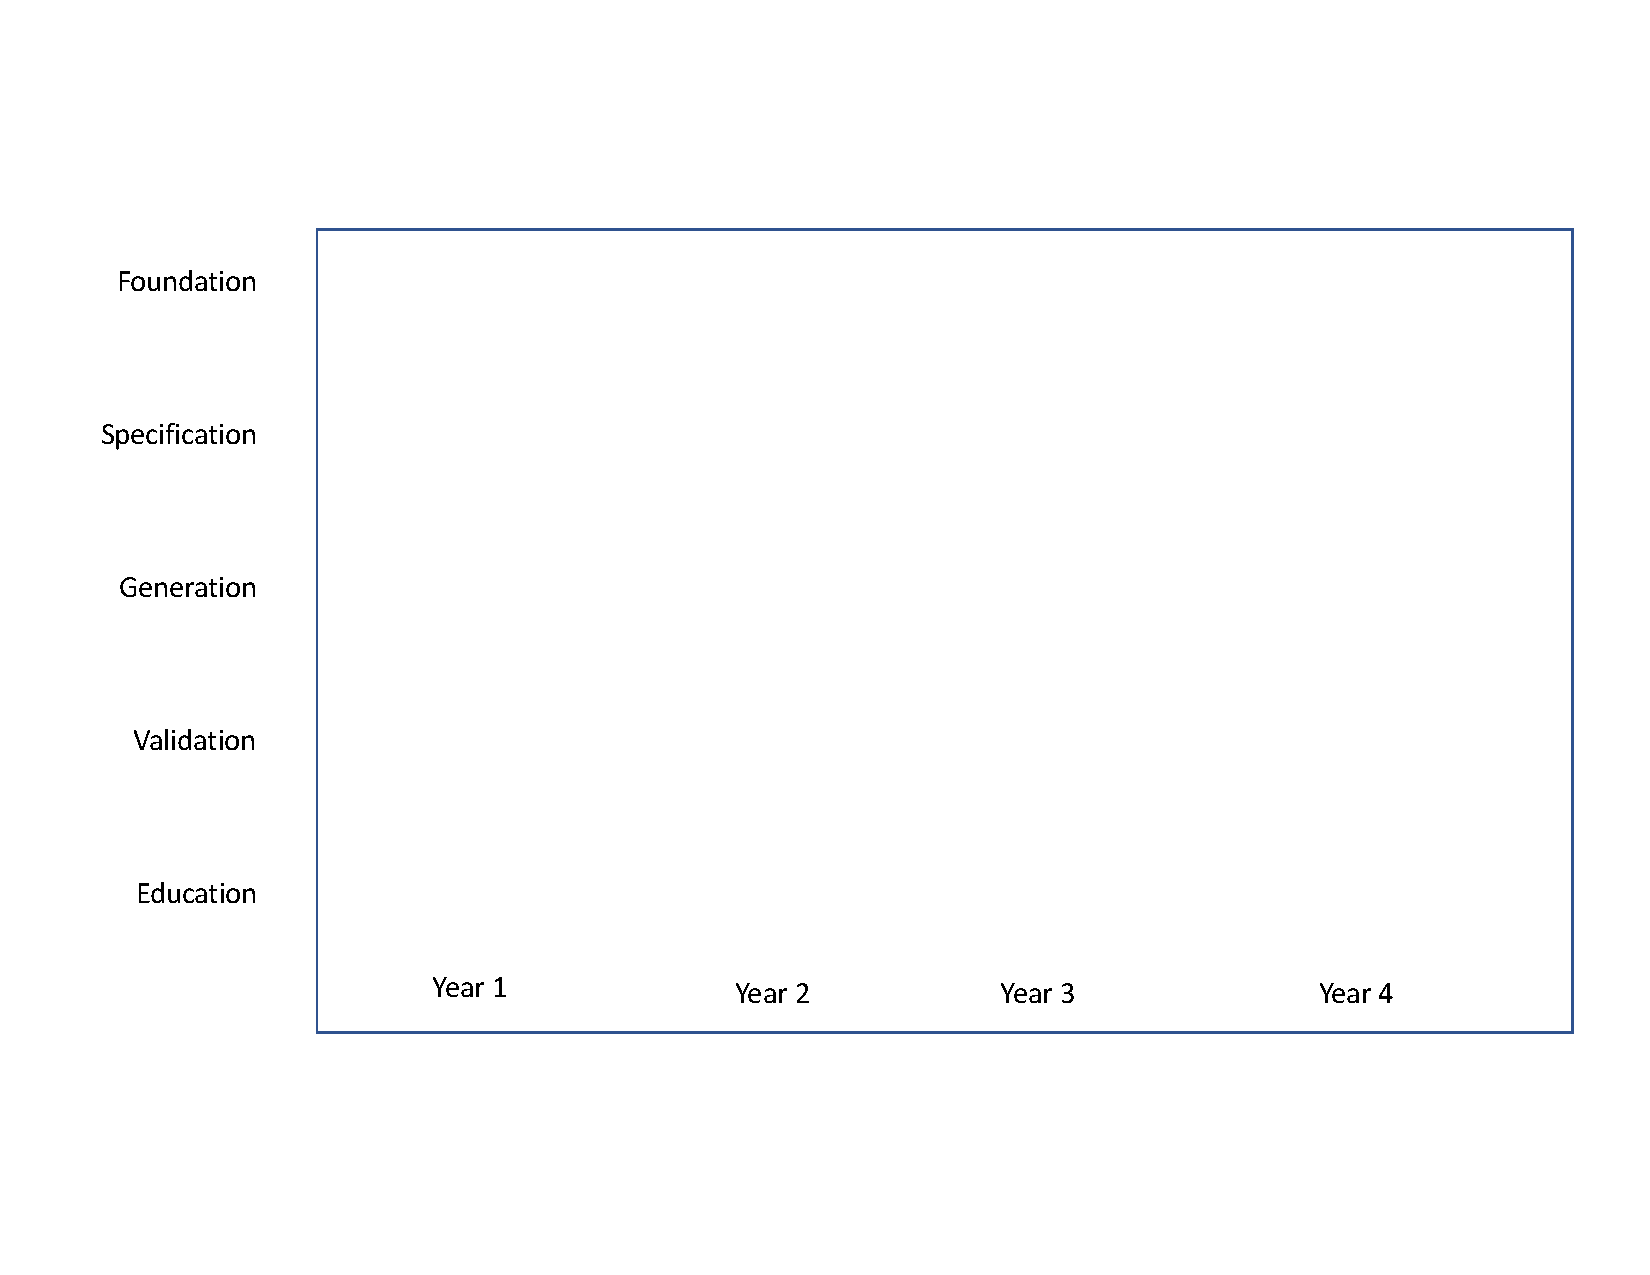
\includegraphics[width=1.1\textwidth]{assets/workplan.pdf}
%   \vspace*{-1.3in}
%   \caption{Plan of work.}\label{fig:workplan}
% \end{figure}

% \vspace*{-.4in}


\SIMPLESECTION{Broader Impacts%
 \pagebudget{.5}}{sec:broader-impacts}

Broad impact is a cornerstone of our research agenda, and many of the
specific tasks we have described---particularly those grouped under
the Diffusion heading (\sectionref{sec:diffusion})---are directly
aimed at broad impacts.  Here we recapitulate those aims and sketch
our plans for mentoring, diversity, and broadening participation in
computing.

\noindent{\bf Impact on industry.} The key area of broad impact from
the proposed work will be ...  \underconstruction{a paragraph about
  tech transfer.} \smallskip

\noindent{\bf Educational Impact.}
%
A second, supportive arena for broad impact will be the
development of educational materials for both students and
professional developers. Educational activities will be
coordinated with the rest of the work, and they are integral to the
project's overall goal of making PBT a standard testing methodology,
readily available to every industrial developer.  Specifically pedagogical
threads within the project are described
in~\sectionref{sec:diffusion}, but we expect many of the tasks
described in other sections will also
influence the design of educational materials.\bcplater{That would be
  stronger if we actually gave section numbers.}

An ancillary educational goal is to
publicize and communicate the benefits of PBT to the broader computer science
research community. As part of these efforts, we will write an article on PBT
for the Communications of the Association for Computing Machinery
(CACM). \iflater\bcp{Mention this article more prominently in the rest
of the document.  Also, promise a CS in Education paper!!}\fi

\smallskip
\noindent{\bf Mentoring and Diversity.}
%
The majority of requested funding will support formative research
experiences and mentoring for graduate students. We
also plan to work with undergraduate and masters students during this project;
they, too will benefit from the research experience. Each graduate
student will have leadership responsibility for multiple facets of the
project, including co-supervising interested undergraduate and masters
researchers.

The PIs will recruit students for this project with a mind towards making
the research area reflective of diversity in the US, and Pennsylvania specifically.
The PIs have had made inroads broadening participation of women in their
groups (1/3 of Pierce's direct Ph.D. mentees and 2/3 of PI
Head's are women). That said, a particular area of focus going forward
will be on increasing representation of
other underrepresented groups, including Black and Latinx students. Pierce (along with Penn colleagues Zdancewic and Weirich)
was recently informed that he will receive funding for an
NSF REU program that will involve 24 undergraduates (8 per
year for three years), selected specifically with an eye to diversity;
we plan to add two more per year specifically to work on this
project. See the Broadening Participation in Computing supplementary
document for more details.

\smallskip
\noindent{\bf Benefits to Society.}
%
The project's goals will also be served by open-source distribution of the tools
built during the project. Key systems will be engineered and documented to a standard
that makes them immediately useful to engineers and students: the projects around
improved generation and shrinking, PBT over logs, and evaluating data
distributions will be particular targets for widespread
dissemination. The remaining projects will be published under a permissive
open source license to serve as models for similar tools for other programming languages and environments.

The project also represents an excellent opportunity for strengthening
collaborations between university researchers and industrial advocates of PBT.  Our
ongoing user study at Jane Street has been carried out with the
enthusiastic support of their developers and management, and we hope
to continue using them as a testbed for prototypes of the tools we
will build.  Similarly, we are in active discussions with the
developers of the Hypothesis, who are keenly
interested in the results of this proposal.\bcplater{Mention Zac's letter,
  either here or elsewhere.  Make sure Hila's and Leo's get mentioned too}
We plan to establish connections with the
developers and user communities of other popular PBT tools such as
ScalaCheck\todolast{citation?}.

Longer term, better testing means better software.  As software
systems have grown to the gigantic scale seen today, good testing
methodologies and tools (unit testing tools, test-first design
methods, etc.) have come to play an ever more crucial role.  Adding a
powerful new testing tool to programmers' arsenals will further boost
this part of the development process, leading to software of every
sort that is more robust, more reliable, and less expensive to build.


% \proposecut{See the Collaboration Plan for
% more.}

% The Project Description must contain, as a separate section within the narrative, a section labeled ``Broader
% Impacts of the Proposed Work". This section should provide a discussion of the broader impacts of the proposed
% activities. Broader impacts may be accomplished through the research itself, through the activities that are
% directly related to specific research projects, or through activities that are supported by, but are complementary to
% the project. NSF values the advancement of scientific knowledge and activities that contribute to the
% achievement of societally relevant outcomes. Such outcomes include, but are not limited to: full
% participation of women, persons with disabilities, and underrepresented minorities in science, technology, engineering, and
% mathematics (STEM); improved STEM education and educator development at any level; increased public
% scientific literacy and public engagement with science and technology; improved well-being of individuals in
% society; development of a diverse,globally competitive STEM workforce; increased partnerships between
% academia, industry, and others; improved national security; increased economic competitiveness of the United
% States; and enhanced infrastructure for research and education.

\SIMPLESECTION{Results from Prior NSF Support\pagebudget{.5}}{sec:prior}

% If any PI or co-PI identified on the project has received NSF funding (including any current
% funding) in the past five years, in formation on the award(s) is required,
% irrespective of whether the support was directly related to the proposal or not.
% In cases where the PI or co-PI has received more than one award (excluding amendments),
% they need only report on the one award most closely related to the proposal. Funding includes not just salary
% support, but any funding awarded by NSF. The following information must be provided:\\

\emph{\underline{PI Pierce}}: (NSF 1955565) ``Collaborative Research:
SHF: Medium: Bringing Python Up to Speed'' (\$437,999,
7/2020--6/2023), with co-PIs Michael Hicks (Maryland) and Emery Berger
(Amherst).
The project aimed to dramatically increase the performance and
correctness of applications written in Python by developing novel
techniques for performance analysis, optimization, run-time systems,
property-based random testing, concolic execution, and program
synthesis. It developed both
novel performance analysis tools and optimizations and novel automatic
testing frameworks. These were largely tailored to and implemented for
Python, but applicable in other, similar languages.
%
{\bf Intellectual Merit.} The project involved work on both
performance measurement (mostly at Amherst and Maryland) and PBT (mostly at Penn
and Maryland).  Specific threads of work involving Penn included
building an early
version~\cite{Frohlich2022} of the Reflective Generators described in
\sectionref{sec:reflective}, carrying out the pilot study of PBT in Python
mentioned in the motivation section
above~\cite{goldstein_problems_2022}, and building on the idea of
freer monads from functional programming to develop ``free
generators,'' which unify parsing and
generation~\cite{goldstein2022parsing}, presented a principled
automatic testing framework for application-layer
protocols~\cite{Li2021:MBToNA}, and developed and released a freely
available mutation testing framework for Python, called {\tt
  pytest-mutagen}~\cite{pytestmutagen}, and applied ideas from
combinatorial testing, a widely studied testing methodology, to modify
the distributions of random test-case generators so as to find bugs
with fewer tests~\cite{DBLP:conf/esop/GoldsteinHLP21}.
%
{\bf Broader Impacts.} Project results and open-source software
products are being used to increase the
performance and correctness of Python applications.
Educational impact has included training both graduate and
undergraduate students, including a female PhD student at Penn, Jessica
Shi.
%
{\bf Publications (involving Penn):} \cite{Frohlich2022,DBLP:conf/esop/GoldsteinHLP21,
  goldstein2022parsing, goldstein_problems_2022, Li2021:MBToNA}.
{\bf Research Products (from Penn)} \cite{pytestmutagen}.

\smallskip

\noindent\emph{\underline{PI Head}} has not previously received NSF support.

% \SUBSECTION{Proposed Study}{}{}
% The Project Description should provide a clear statement of the work to be undertaken and must include:
% objectives for the period of the proposed work and expected significance; relation to longer-term goals of the PI's
% project; and relation to the present state of knowledge in the field, to work in progress by the PI under other
% support and to work in progress elsewhere.
%
% The Project Description should outline the general plan of work, including the broad design of activities to be
% undertaken, and, where appropriate, provide a clear description of experimental methods and procedures.
% Proposers should address what they want to do, why they want to do it, how they plan to do it, how they will
% know if they succeed, and what benefits could accrue if the project is successful. The project activities may be
% based on previously established and/or innovative methods and approaches, but in either case must be well
% justified. These issues apply to both the technical aspects of the proposal and the way in which the project may
% make broader contributions.

\iflater
\section*{Stuff to think about once the document stabilizes}

\todo{GPG: To increase the diversity of the reviewer pool, CISE actively encourages each proposer to include a list of suggested reviewers (including email addresses and organizational affiliations) whom they believe are especially well qualified to review the proposal and are not conflicted with project personnel. Suggestions for reviewers from groups underrepresented in computing are especially encouraged. Proposers should follow the guidance in PAPPG Chapter II.D.1.}

\todo{GPG: Issues of fairness, ethics, accountability, and
  transparency (FEAT) are important considerations for many core
  topics in computer and information science and engineering. In
  projects that generate artifacts ranging from analysis methods to
  algorithms to systems, or that perform studies involving human
  subjects, PIs are encouraged to consider the FEAT of the outputs or
  approaches.  (We should touch on this point somewhere.)}

\todo{Does it make sense to include something about separation logic,
  or more generally about ``generators with difficult preconditions''?
 Could be speculative, as long as it's not vacuous.}

\bcp{I see quite a few little issues in the citations.  Let's make
  sure we give that a quick polishing pass.}

\bcp{We could / should read some past funded NSF Large proposals for
  ideas about how people talk about their work.}

\todo{Remember to turn off all the ``forreaders'' stuff.}

\todo{Make sure the intro to each section accurately reflects what's
  in the section, and in which order.}

\todo{Every section (including the broader impacts and each of the
  research sections) needs to explicitly address how we will measure
  success...  Check that we've done this.}

\discuss{Make sure readers can identify a Related Work section.}

\discuss{Get letters from Leo and Hila.
  \begin{itemize}
  \item A letter of collaboration from any entity not receiving funds
  from the project budget should be provided at the time of submission
  of the proposal. Such letters should appear on the organization’s
  letterhead and be signed by the appropriate organizational
  representative. These letters must not deviate from the restrictions
  and requirements set forth in the NSF PAPPG Chapter II.D.2.  (Done,
  I think.)
  \item Any substantial collaboration with individuals not included in
  the budget should be described in the Facilities, Equipment and
  Other Resources section of the proposal (see Chapter II.D.2.g) and
  documented in a letter of collaboration from each collaborator. Such
  letters should be provided in the supplementary documentation
  section of Research.gov and follow the format instructions specified
  in Chapter II.D.2.i. Collaborative activities that are identified in
  the budget should follow the instructions in Chapter II.E.3.  (Needs
  done.)
  \item We also need to make sure that the appropriate sections of the
  project description mention the collaborations.
  \end{itemize}
}

\fi

\bigskip \forreaders{Don't miss all the supplemental documents beyond
  the bibliography that we'd love to hear your comments on...}
